\documentclass[11pt,a4paper]{article}
\pdfminorversion=7
\usepackage[utf8]{inputenc}
\usepackage[T1]{fontenc}
\usepackage{amsmath,amssymb,amsfonts,amsthm}
\usepackage{graphicx}
\usepackage{hyperref}
\usepackage{geometry}
\usepackage{enumitem}
\usepackage{booktabs}
\usepackage{natbib}
\usepackage{microtype}
\usepackage{xcolor}

\geometry{
    a4paper,
    total={170mm,247mm},
    left=20mm,
    top=25mm,
}

\hypersetup{
    hidelinks,
    pdfstartview={FitH},
    pdftitle={Refractive Gravity: An Ontological Picture and the Foundations of Mathematical Formalism (Version 3.5)},
    pdfauthor={George Lotishvili}
}

\newcommand{\RefG}{\mathrm{RefG}}

\title{\textbf{Refractive Gravity: An Ontological Picture and the Foundations of Mathematical Formalism}\\[0.5em]\large Version 3.5}
\author{\textbf{George Lotishvili}\\
\small Associate Professor, East European University\\
\small Tbilisi, Georgia\\
\small \href{mailto:g_lotishvili@eeu.edu.ge}{\texttt{g\_lotishvili@eeu.edu.ge}}}
\date{2026}

\begin{document}

\maketitle

\begin{center}
\textbf{Zenodo DOI:} \href{https://doi.org/10.5281/zenodo.21325652}{10.5281/zenodo.21325652}
\end{center}

\begin{abstract}
Refractive Gravity ($\RefG$) develops a relational account of measurement in which clocks, rulers, light, and observers are physical constituents of the system being measured. A single pre-spatial foundation gives rise, through resonant self-distinction, to operational space, time, matter, and gravitational geometry. Stable massive matter is represented by locally self-confined nonlinear wave structures, or oscillons, whose dynamics establish pressure deficits in the manifested medium. On the common-scaling branch, the externally measured ruler scale and mass, together with the clock rate, scale as $p$, while the coordinate speed of light scales as $p^2$. In the specified low-energy class of the post-Genesis relational-coframe action, the TEGR coefficients follow, and the torsion--curvature identity gives the Einstein--Hilbert action up to a boundary term. The standard PPN vector is recovered under the stated complete 1PN conditions. A covariant clock--label--response action also admits an exact exponential static exterior; a regular $C^2$ kinematic core provides a target for the interior source problem. The quadratic expansion of the oscillon amplitude--phase action about its strict vacuum is the free complex Klein--Gordon action on the same coframe. On a fixed Minkowski background, canonical quantization of this sector yields positive-energy particle and antiparticle sectors in bosonic Fock space, with mass $m$ and spin zero for the vacuum excitations. In the cosmological description, increasing inter-node separation lowers the background pressure and material scale, and internal measurements determine the operational scale factor $A=a/p$. The monograph presents the conceptual framework and its physical interpretation. Published formal calculations are archived on Zenodo; the final section distinguishes established results, their domains of validity, and the remaining problems.
\end{abstract}

\newpage
\tableofcontents

\vfill
\begin{center}

\includegraphics[width=0.34\textwidth]{figures/logo.pdf}
\end{center}
\vfill

\newpage

\section*{Preface}
\addcontentsline{toc}{section}{Preface}

Refractive Gravity ($\RefG$) takes a relational principle of measurement as its starting point: clocks, rulers, light, and observers belong to the same physical world, and measurements are made using material standards within that world. On this basis, the monograph develops a unified ontological account of a single foundation and the geometry, matter, and time that emerge from it. In the specified low-energy limit, the same relational coframe supports Einstein--Hilbert geometry, while the quadratic sector of the oscillon action about its strict vacuum is a free complex scalar quantum field on that coframe. A covariant action for the clock, material labels, and deficit field also admits an exact exponential static exterior. The text presents the conceptual analysis and physical interpretation; the published formalism and calculations are available in the public scientific archive on Zenodo \citep{lotishvili2026a,lotishvili2026b}.

The subjects addressed in this monograph are at different stages of development. Some results have been derived and tested formally; others are specified physical constructions or directions for further mathematical development within the same framework. The final section, \emph{Current Status of the Research Program}, summarizes the results, their conditions of validity, and the unresolved problems.

\section*{Introduction}
\addcontentsline{toc}{section}{Introduction}

General relativity and quantum field theory are the two principal frameworks of modern fundamental physics. Einstein's general relativity describes gravity as the dynamical geometry of spacetime. Quantum field theory usually describes matter and gauge interactions through operator-valued fields on a prescribed background.

Both theories have extensive experimental support, but they use different underlying structures. Spacetime geometry is dynamical in general relativity, whereas the usual formulation of quantum field theory assumes a specified background geometry and time parameter.

Several unresolved problems bear on the construction of a unified description:
\begin{enumerate}[label=\arabic*.]
\item \textbf{The Singularity Problem:} Classical descriptions of black holes and the cosmological origin lead to geodesic incompleteness and, in important cases, divergent curvature, indicating a limit of validity of the classical description.
\item \textbf{Astrophysical and Cosmological Anomalies:} Within the standard cosmological model, galactic rotation curves, the Radial Acceleration Relation (RAR), and the Baryonic Tully--Fisher Relation (BTFR) are described through dark-matter halos together with baryonic galaxy-formation physics, while accelerated cosmic expansion is attributed to a vacuum-energy cosmological-constant term. A naive continuation of field theory to a Planck-scale cutoff may exceed the observed vacuum density by roughly 120 orders of magnitude.
\item \textbf{Structural and Hierarchical Problems:} Quantum-measurement randomness and the arrow of time lack a unified structural explanation. The pronounced hierarchy of charged-lepton and quark masses, the values of dimensionless constants---including $\alpha \approx 1/137$---and the weakness of gravity relative to the electroweak scale ($M_{\rm Pl}/v_{\rm EW} \sim 10^{17}$) enter the standard framework as empirical features without a common explanation.
\end{enumerate}

The search for a common physical foundation has taken several forms. Einstein pursued a geometric unification of electromagnetism and matter throughout his later life. John Archibald Wheeler investigated the relations among geometry, matter, and information through the concepts of \textit{Mass without Mass} and \textit{It from Bit} \citep{wheeler1955,wheeler1990}.

Andrei Sakharov proposed an elastic interpretation of gravity induced by quantum vacuum fluctuations \citep{sakharov1967}. Ted Jacobson derived Einstein's equations from a thermodynamic equation of state for local horizons \citep{jacobson1995}. Erik Verlinde described gravitational attraction as a holographic entropic force \citep{verlinde2011}, while Roger Penrose related the causal structure of spacetime to gravitational collapse through his singularity theorem \citep{penrose1965}.

These approaches use different mathematical formalisms. The ontological question examined here is whether space, time, gravity, and the particle spectrum can be described as dynamical manifestations of a single underlying foundation.

The monograph develops the conceptual and ontological framework of \textbf{Refractive Gravity ($\RefG$)} to address this question.

\subsection*{Operational Foundations and Three Fundamental Principles}
\addcontentsline{toc}{subsection}{Operational Foundations and Three Fundamental Principles}

Established physical formalisms generally assume specified measurement procedures and structures, including smooth coordinates, a time axis, and field operators. $\RefG$ extends Percy Bridgman's operationalism \citep{bridgman1927} by examining the physical prerequisites of measurement itself: the processes that establish local distinguishability and thereby make material rulers and clocks possible.

In 1905, Einstein rejected absolute time and defined simultaneity operationally using clocks and light signals \citep{einstein1905}. $\RefG$ seeks to describe the physical mechanism that produces the stable clock, material particle, and propagating signal on which such measurements depend.

The framework is based on three fundamental postulates:
\begin{enumerate}[label=\arabic*.]
\item \textbf{Monistic Ontological Foundation:} Nature has one universal foundation from which spatial relations and physical timekeeping emerge. Its resonant self-distinction produces a manifested medium whose phase, pressure, shear, rotational, and topological modes correspond to elementary fields, forces, and particles.
\item \textbf{The Oscillon Nature of Matter:} A stable massive material unit is an \emph{oscillon}: a locally self-confined, self-sustaining nonlinear wave configuration of the manifested medium. Massless carrier modes are freely propagating waves in the same medium. Intense internal oscillation establishes a persistent static pressure-deficit profile around the oscillon.
\item \textbf{Gravity as Effective Refraction:} Oscillon matter establishes an inhomogeneous pressure deficit in the medium. The deficit changes the effective geometry, in which light and matter waves undergo refractive deflection. $\RefG$ thus assigns a physical refractive mechanism to gravitational curvature. In the relational-coframe description, the pressure deficit is the volumetric scalar readout of the full local geometry. Symmetric deformation and shear determine the tensor structure of gravity, while frame orientation is an inertial gauge freedom.
\end{enumerate}

\subsection*{Lorentz Invariance and Historical Precedents}
\addcontentsline{toc}{subsection}{Lorentz Invariance and Historical Precedents}

The Michelson--Morley experiment of 1887 detected no aether wind associated with the Earth's motion and placed stringent constraints on 19th-century models of a stationary luminiferous aether independent of matter \citep{michelson1887}. The $\RefG$ foundation-medium belongs to a different ontological class: measuring instruments, observers, and light are collective wave excitations of the same medium.

Because observers, apparatus, and light are collective excitations of the same medium, uniform translational motion is described as a symmetric phase translation of the wave configuration. On the Lorentz-covariant branch, this motion is lossless and produces no aether-wind effect. The conceptual connection to Lord Kelvin's vortex-atom hypothesis \citep{thomson1867} is the representation of \textbf{matter as an organized form of motion in the medium itself}.

\newpage
\subsection*{Eight Principal Topics}
\addcontentsline{toc}{subsection}{Eight Principal Topics}

This text sets out the ontological foundations of $\RefG$ and connects the computational formalism archived on Zenodo with its physical interpretation. Medium-based unification has precedents, including Winterberg's Planck-aether model \citep{winterberg2002}. The distinctive starting points of $\RefG$ are the emergence of measurability and the population-level resonant stabilization of matter.

The monograph addresses eight interconnected topics:
\begin{enumerate}[label=\arabic*.]
\item \textbf{The Emergence of Time and a Common Oscillon Clock Rate:} In the Genesis scenario of $\RefG$, time begins with a centerless transition encompassing the whole foundation. The first distinguishable relations establish an ordering of events; oscillon seeds and subsequently stable matter form within the resulting network. Local pressure changes rescale the particle spectrum through the common frequency scale $\Omega_t$, while the oscillon's internal structure is encoded in the dimensionless labels $s_i$ and their ratios.
\item \textbf{Two-Channel Mass Accounting:} The oscillon's internal topological state describes its conserved energetic store; externally read gravitational mass is the integral response of the pressure deficit established in the medium. Separating these two channels prevents the same energy from being counted twice.
\item \textbf{Biconformal $p/p^2$ Scaling and the Complete 1PN Response:} The external footprint of a local ruler, externally read mass, and clock rate follow $p$, whereas coordinate light speed follows $p^2$. In the static spherical weak field this geometry gives $\gamma=1$. With a canonical gradient term, linear coupling to the active source density entering Gauss's law, and no additional unsuppressed term at the same order, the logarithmic response $u=-\ln p$ also gives $\beta=1$. In the corresponding low-energy class of the post-Genesis relational-coframe action, the TEGR coefficients are obtained, and the exact torsion--curvature identity converts the action to Einstein--Hilbert form. When the complete 1PN conditions are satisfied, the standard PPN vector follows.
\item \textbf{One Coframe for Gravity and Free Quantum Matter:} The vacuum quadratic sector of the nonlinear oscillon amplitude--phase action takes exactly the form of the free complex Klein--Gordon action on the same relational coframe. On the fixed Minkowski branch, standard canonical quantization of this quadratic sector yields positive-energy particle and antiparticle sectors of bosonic Fock space, a conserved global phase charge, microcausality, mass $m$, and spin zero for the free excitations about that vacuum. Einstein--Hilbert geometry and standard free quantum matter are thereby placed on one operational geometry.
\item \textbf{The Koide $C_3$ Phase Geometry:} A three-phase map in charged-lepton square-root mass space reproduces Koide's $K=2/3$ identity exactly when $A_K=\sqrt2$. $\RefG$ reads this geometry as a candidate imprint of a ninth-order return cycle in which $h=2$ fixes the phase angle $\theta=2/9$.
\item \textbf{The Nodal Origin of the Fine-Structure Constant ($\alpha$):} The fine-structure constant $\alpha \approx 1/137$ is read as the dimensionless ratio between the electric-flux and transverse-photon responses of one nodal network. Both channels transform together, leaving their ratio invariant.
\item \textbf{Genesis, Foundation Expansion, and Its Internal Readout:} The first distinguishable relations begin time; resonant coupling connects the network; stable matter, radiation, and long-term relaxation take form in subsequent phases. In the post-Genesis realization, growth of the foundation's inter-node scale lowers $P_F$, and the pressure decline reduces the material scale $p$. A neutral collective phase charge is distributed through the expanding three-dimensional volume: its conservation gives $\eta_Fa^3=1$, while homogeneous constitutive relations yield $P_F/P_{F,0}=a^{-3}$, $p=a^{-3/2}$, and $A=a/p=a^{5/2}$. Accordingly, the internally measured $A$ uniquely reconstructs the normalized relative scales: $a=A^{2/5}$, $p=A^{-3/5}$, and $\eta_F=A^{-6/5}$. The variables $p_C$ and $P_F$ describe distinct physical quantities; their constitutive relation belongs to the microphysics of the foundation. On the ideal homogeneous background, $A$ unifies redshift, signal time dilation, and geometric distances in one response. When the cold phase source couples to the plasma only through the common geometry and the local dimensionless atomic and QED ratios retain their standard values, the CMB initial-value problem on this same $A$ geometry takes exactly the standard Einstein--Boltzmann, recombination, and line-of-sight form.
\item \textbf{Two Readouts of a Single Spectral Operator---A Central Hypothesis:} The short-wavelength eigenfunctions of a unified volumetric Helmholtz/Laplace-type resonator are read as microscopic particle modes, whereas its long-wavelength modes are read as the macroscopic structure of the cosmic web and galaxy clusters.
\end{enumerate}

\subsection*{Historical Lineage and Priority Boundaries}
\addcontentsline{toc}{subsection}{Historical Lineage and Priority Boundaries}

Individual mechanisms in $\RefG$ are related to the following theoretical approaches:
\begin{itemize}
\item The $p/p^2$ scaling law is related to the Polarizable Vacuum (PV) approaches of Robert Dicke and Harold Puthoff \citep{dicke1957,puthoff2002}; $\RefG$ ties it to the ontology of a nodal network and two-channel mass accounting.
\item The three-phase geometric reading of Koide's formula extends the work of Carl Brannen and Robert Foot \citep{brannen2010,foot1994}, while the holonomic origin of $2/9$ is related to the closed family cycles studied by Konstantin Shulga \citep{shulga2026}. $\RefG$ combines this structure with the $\theta$-blindness argument and the $C_3$ symmetry of a three-dimensional volumetric resonator.
\item The historical motivation for background-pressure relaxation and a possible microscopic origin of $\Lambda$ comes from the $q$-theory of Klinkhamer and Volovik \citep{klinkhamer2008}; $\RefG$ writes the background dynamics of its selected branch in Einstein--Hilbert geometric language. The motivation for three spatial dimensions is connected with studies of topological knotting and stability in nodal structures \citep{whitrow1955,berera2017}.
\end{itemize}

$\RefG$ combines these approaches within a single causal framework, connecting the emergence of operational measurability and oscillon mass with galactic vortical flow and cosmological horizons.

The following chapters examine the physical content of these mechanisms and the relations among them.

\section{The Ontological Foundation}

\subsection{A Single Foundation and Its Manifested Medium: Substance, Void, and the Dynamics of Existence}

Modern fundamental physics describes the Universe as a system of distinct, interacting quantum fields. The Standard Model relates these fields through common gauge symmetries, internal degrees of freedom, and interaction rules. Refractive Gravity ($\RefG$) associates this diversity with a single postulate: \textbf{nature has one universal, pre-spatial ontological foundation.} Its resonant self-distinction produces a measurable medium with multiple response channels. Fundamental fields, gauge interactions, and elementary particles correspond to its topological, phase, pressure, shear, and rotational modes. The term \emph{foundation-medium} denotes this self-distinguished, physically manifested state of the foundation.

This monistic account has theoretical precedents. In 1870, William Kingdon Clifford proposed that matter corresponds to small, moving regions of spatial curvature \citep{clifford1876}. $\RefG$ connects this geometric interpretation to a physical mechanism: the self-distinguished medium supports pressure, shear, hydrodynamic, and resonant responses as well as geometric curvature.

A clear theoretical precedent for the emergence of distinct particle and gauge sectors from one carrier is the string-net condensation model of Michael Levin and Xiao-Gang Wen \citep{levin2005}. In that framework, collective many-body entanglement produces structural analogues of gauge bosons and fermionic excitations. Levin--Wen begins with a prestructured quantum lattice; $\RefG$ associates the same unifying potential with the self-distinction of one universal pre-spatial foundation.

The description of the Universe as a unified continuous medium involves two asymptotic limits in the $\RefG$ dynamical picture:
\begin{enumerate}[label=\arabic*.]
\item \textbf{The Absolute Maximum of Substance:} A saturation limit characterized by maximal pressure, mass--energy potential, and operational nodal density.
\item \textbf{The Zero-Distinguishability Bound:} A limit in which interaction and physical measurability vanish entirely.
\end{enumerate}

The void is the logical limit at which physical distinguishability vanishes. In this account, physical reality consists of bounded, nonlinear oscillatory dynamics between the two limits. Stable local units of the foundation, termed \emph{nodes of existence}, form within this domain.

The reference background $\varphi = 0$ is the quiescent yet physically active state situated between these two extrema. At the limit of zero distinguishability, nodal interactions and measurable traces completely vanish; $\varphi = 0$ designates the unperturbed baseline state of the manifested medium.

The manifested medium supports multiple dynamical responses: volumetric compression, topological twist, vortical flow, and transverse wave excitation. Its phase, pressure, shear, and topological degrees of freedom together provide the physical basis to which $\RefG$ relates electric charge, spin, and the particle spectrum.

The unperturbed state of the foundation-medium, denoted by $\varphi=0$, is its background vacuum regime. The foundation is present throughout the manifested medium; the excitation level, operational density of distinguishable nodes, and coupling strength vary locally. Increasing the operationally unmeasurable intervals between nodes rarefies the foundation and lowers its pressure state.

Here pressure is the effective pressure--energy state variable of $\RefG$. The unperturbed background is $\varphi=0$; $\varphi>0$ is the elevated pressure--energy branch (compression), and $\varphi<0$ is the deficit branch (rarefaction). The gravitational readout is built on the gradient profile of the deficit branch. Classical Bernoulli pressure is its immediate physical analogue: an external observer reads a local change in $\varphi$ as a change in clock rate, coordinate signal propagation, operational size, and effective gravitational mass.

\subsection{From Unity to Multiplicity: The Emergence of Measurability and Operational Space}

The Genesis postulate of $\RefG$ assumes an initially undifferentiated foundation, before change, event order, duration, or geometry has emerged. The origin of the Universe is the first physical event and the starting point for measuring time.

The origin scenario developed here is a centerless transition encompassing the whole foundation. It specifies a common initial condition with no preferred spatial center. Space, physical distance, propagation speed, and an exterior acquire meaning only through the connections produced by that transition.

At this boundary the foundation first produces minimally distinguishable relations. Event order and both measures of time begin here, at $t=0$ and $\tau=0$. This initial layer of distinguishable connections is the minimal network of existence; material particles and stable oscillons form during its subsequent development.

Nonlinear modes localize on the first relations as oscillon seeds. Their resonant fields spread across the relational layer and overlap. Once the physical threshold of distinguishability is crossed, this overlap binds operationally separate regions into a single network. The causal sequence therefore begins with the first relation and continues through localization and network coupling. Local locking and global coupling may be partly contemporaneous; their precise ordering is set by resonant dynamics and the physical coupling threshold.

In the Genesis scenario, the Universe is an interconnected network with no boundary or preferred center. A finite periodic graph provides a simple mathematical model: it is finite and connected without any node being a unique center. The structure of the foundation's connections determines the dimension and topology of the physical Universe.

The energy of the initial coherent state is distributed among oscillon seeds, their resonant fields, freely propagating waves, a thermal sector, and the collective deformation of the foundation. A continuity law accounts for energy in each sector and the fluxes between them in a common balance: a loss in one sector is a gain in another. The phase energies and equation of state determine the direction of this redistribution.

The first collective change initiates the foundation's self-distinction. Operational space becomes measurable when a stable relation between nodes reaches the minimum distinguishability scale $\ell_*$. An interval between distinguishable nodes provides the elementary basis of physical space. A delay in signal transfer establishes measurable duration, while the local energetic strain associated with self-distinction provides the proposed ontological precursor of mass. The integrated response of the deficit profile that this strain produces in the surrounding foundation is subsequently measured as gravitational mass.

Physical interpretation requires comparison. At the ontological origin, three inseparable elements are identified:
\begin{itemize}
\item \textbf{Node:} A locally distinguishable, discrete state of the foundation;
\item \textbf{Trace:} The energetic and phase alteration imparted by a node to the surrounding medium;
\item \textbf{Relation:} The operational capacity to compare one local state with another.
\end{itemize}

The relations among these three elements establish the operational network whose macroscopic properties are described as space, time, and matter.

A completely undifferentiated foundation has a single, indivisible identity. Its resonant self-distinction produces the first persistent difference and establishes the physical basis for quantity and counting. Distinguishable manifestations constitute separate physical units, while the foundation itself remains indivisible: multiplicity consists of stable, mutually distinguishable states of one identity.

The primary unit of measurement is a preserved relation. In an undistinguished state, no second entity exists for comparison. Self-distinction yields two distinct states of the same foundation and establishes the primary link between them; here begin counting, spatial extension, and the relative ordering of events.

In an informational description, the first persistent distinction is analogous to a bit: a distinguishable trace is represented by 1, and its absence in the specified relation by 0. Different arrangements of these two states form complex structures, just as mutually distinguishable states of the foundation give rise to the diversity of the measurable Universe.

Persistent self-distinctions of a single foundation generate locations that can be counted and compared. Multiplicity is described in terms of different distinguishable states of one primary identity. The foundation itself is considered outside time; the age of the measurable Universe refers to the sequence of events that emerges from it.

This account places observers within the physical system they measure. Observers and their instruments are complex, composite wave structures of the same nodal network. Bridgman's operationalism defines a physical concept through the set of operations by which it is measured \citep{bridgman1927}. $\RefG$ seeks an ontological basis for this principle by examining the physical conditions that make those operations possible.

The measurable Universe is described as an ongoing process of self-distinction in the foundation-medium. Operational space emerges from physically distinguishable relations. The universal foundation may also exist beyond the domain of such relations, but it is manifested as a physical object only where it has an operationally measurable effect.

Absolute inter-node separation cannot be measured directly because the observer has no absolute ruler external to the medium. Only its operational effects are measurable. Operational space emerges when the relation between at least two nodes becomes physically distinguishable. Below this threshold, a difference remains part of the foundation's local internal state; above it, the difference is registered through changes in clock rate, operational size, mass, and signal propagation.

$\RefG$ introduces a dynamic lower bound of minimal operational distinguishability, denoted by $\ell_*$:
\begin{itemize}
\item At scales smaller than $\ell_*$, no independent measurable relation can form (information is indistinguishable);
\item At the scale $\ell_*$, the first stable, physically distinguishable record emerges;
\item At scales larger than $\ell_*$, inter-node intervals register as changes in pressure, clock rates, and signal propagation.
\end{itemize}

The physical rationale for this bound is the finite resolution required by a stable record. The Planck length $\ell_{\rm Pl} = \sqrt{\hbar G/c^3}$ is a dimensional scale constructed from fundamental constants, whereas $\ell_*$ is the dynamical threshold for stable record formation. Their relation is fixed by the microdynamics of the foundation.

The ontological origin of the Universe is a completely undifferentiated primary foundation-state. A geometric point is already a concept of formed space; two distinguishable points and the extension between them arise together with the operational inter-node interval. An asymmetry formed in the foundation-medium leaves a stable trace, the relation becomes readable, and multiplicity and geometry emerge in the same event.

$\RefG$ connects this operational description to gravity. A spatial gradient in the pressure state of the foundation-medium produces coordinated changes in clock rate, operational size, and coordinate signal propagation, which together define the gravitational geometry. A homogeneous change produces a common background recalibration; acceleration and refractive deflection arise from spatial inhomogeneity.

\subsection{Nodal Transmission: Waves, Time, and Self-Calibration}

The foundation's first collective change creates a minimal relational layer. Each node is a functionally distinguishable state that preserves the trace of a physical change and can relay it to adjacent nodes. Subsequent transmission, together with resonant coupling produced by overlapping resonant fields of oscillon seeds once the distinguishability threshold is crossed, joins this layer into an operational network. Spatial proximity and operational distance emerge from the stable organization of these physical couplings.

A wave in this network is the sequential transmission of state and phase. Light is a freely propagating transverse phase trace, whereas an oscillon is a locally self-confined, self-sustaining configuration of the same transmission mechanism. When matter moves, this localized wavepacket is transferred from node to node, reconstructing its phase integrity at each successive location. Light and matter are thus the propagating and localized modes of a single medium.

The foundation's first complete self-distinction establishes an initial ordering of events and the origin of time. Each subsequent transmission in the network extends that sequence. Recurrent phase relations establish a rate for physical processes, and comparisons among stable oscillon cycles make clock measurements possible. The local rate of time is determined jointly by the rate of state transfer through the network and the frequency at which an oscillon completes its own cycle.

$\RefG$ relates the rate of state transfer between nodes to their density and coupling strength. Rarefaction slows this transfer and reduces the rate of material processes with respect to coordinate time.

The observer's body, clocks, rulers, light, and matter are modes of the same medium. In a pressure-deficit region, nodal density, transmission rate, oscillon period, and operational size change together. Local measuring devices adjust to the same environment. An observer using local units therefore measures the usual clock rate and size, and an unchanged local speed of light ($c$); comparisons between processes in different environments reveal differences in time, size, and mass.

On the physically admissible low-energy branch, transmission is isotropic, non-dissipative, and Lorentz invariant: the local speed of light is unchanged, and uniform motion experiences no friction.

\subsection{Common Local Clock Rate and Resonant Locking}

The emergence of time and the establishment of a common local clock rate are distinct stages. In the Genesis scenario, time begins with the first foundation-wide self-distinction. A common local rate is established later, when the intrinsic frequencies of stable material oscillons acquire fixed, persistent ratios. In this collective state, internal coordination and nonlinear locking within the local network determine the rate of time, as in Kuramoto-type synchronization.

The network's normal modes and the physical basis of material clocks emerge as its connections form. The resulting medium is treated as a volume resonator: its coupling operator and boundary conditions determine the spectrum of admissible modes. The three-dimensionality of this resonator is part of the physical model of $\RefG$.

Elementary-particle frequencies are determined by mutual balance and coordination within the foundation's collective dynamics. The foundation specifies the space of admissible modes, and interactions among particle modes establish a stable, resonantly locked state within that space.

Pressure changes the network's common frequency scale with respect to coordinate time. We denote this scale by $\Omega_t(x)$; the subscript $t$ specifies frequency per unit of the foundation's coordinate time. The common response to pressure is
\begin{equation}
\frac{\Omega_t(x)}{\Omega_{t,0}}=p(x),
\qquad
d\tau=p\,dt.
\end{equation}
Here $\tau$ is the process time measured by material clocks. As $p$ decreases, fewer material cycles occur within a fixed coordinate-time interval $dt$. A local observer uses a $\tau$ clock and measures the usual local rate; differences arise when environments or epochs are compared.

The oscillon's internal geometry distinguishes its stable modes by dimensionless structural labels $s_i$. Their relation to the common frequency scale is
\begin{equation}
\nu_i^{(t)}(x)=s_i\,\Omega_t(x),
\qquad
\nu_i^{(\tau)}=\frac{\nu_i^{(t)}}{p}.
\end{equation}
The labels $s_i$ characterize the oscillon's internal spectrum, whereas $\Omega_t$ is the environmental frequency scale defined with respect to coordinate time. A common pressure change rescales the entire spectrum by one factor; the process clock compensates locally for this common change. The labels $s_i$ and their invariant ratios distinguish the particle modes.

In a low-pressure region, the coordinate-time frequency scale $\Omega_t$ decreases. Inter-node transfer is more frequent in a dense, high-pressure foundation; in a rarefied foundation, coupling and material processes evolve more slowly with respect to coordinate time. Delayed inter-node signal transfer, a lower pressure--energy state, and a reduced $\Omega_t$ are three operational manifestations of the same network state. Each is counted once in the quantitative causal description.

Local clocks and atomic processes adjust to the medium, so observers measure the usual rate using their own local standards. The common rescaling preserves dimensionless ratios; the observed stability of the fine-structure constant is a stringent test of this principle. In this account, particle mass ratios originate in the internal $s_i$ spectrum of oscillons.

Ernst Mach's principle is a historical precursor of this relational approach \citep{mach1883}. $\RefG$ gives it a local dynamical interpretation: the common clock rate is determined directly by the collective state of the local resonant network, with the influence of distant masses encoded in that state. Relationality and local causality are therefore properties of the same network.

In $\RefG$, the fine-structure constant $\alpha \approx 1/137$ is interpreted as an invariant dimensionless ratio of the electric-flux and transverse-photon responses of the nodal network. Under common rescaling, it remains unchanged as local pressure varies.

A receiver measures a light signal against its local atomic standard. For stationary emitters and receivers in a static gravitational field, the locally measured frequencies satisfy
\begin{equation}
\frac{\omega_o}{\omega_e}=\frac{N_e}{N_o},
\end{equation}
where $N$ is the static lapse. On the selected common-response branch, $N=p$, so a signal climbing from a pressure-deficit region to a distant observer has $\omega_o/\omega_e=p_e/p_o<1$: it is gravitationally redshifted.

On the homogeneous cosmological branch, comoving emitters and receivers instead obtain
\begin{equation}
\frac{\omega_o}{\omega_e}=\frac{A_e}{A_o},
\qquad
1+z=\frac{A_o}{A_e}=\frac{a_o/p_o}{a_e/p_e}.
\end{equation}
Both results follow from propagation in the corresponding operational metric and measurement by local clocks. The common pressure response is included once in each description; the static and cosmological formulas apply to different propagation conditions.

In $\RefG$, the rate of time is a property of the local resonant network's ontological state. Pressure changes rescale the network and all compatible processes by a common factor, preserving their dimensionless ratios. Every measurement is performed within the same physical network, whose processes give time its physical meaning.

The stability of dimensionless ratios provides an empirical test of this principle: \textbf{a reliably established nonzero $\Delta\alpha/\alpha$ correlated with a change in local pressure would falsify the population-level common-clock-rate postulate.}

\subsection{Oscillons, Pressure Deficits, and the Origin of Mass}

$\RefG$ describes the electron, proton, and quark as \textbf{oscillon modes}. An oscillon is a locally self-confined, self-sustaining nonlinear wave structure in the foundation-medium: a coherent oscillatory state of the medium itself.

Lord Kelvin's vortex-atom hypothesis is a historical precursor \citep{thomson1867}. The shared conceptual principle is that a particle is a self-confined, dynamical topological configuration of the medium. The oscillon description develops this idea within nonlinear field theory and topology.

Intense internal oscillation, rotation, or localized energy confinement in an oscillon lowers the static pressure of the surrounding foundation-medium. Bernoulli's classical hydrodynamic balance provides an analogue \citep{bernoulli1738}: \textbf{under the appropriate conditions for stationary flow, an increased dynamical contribution is accompanied by a decrease in static pressure.} On the weak, static gravitational branch of $\RefG$, the corresponding schematic pressure--energy relation is
\begin{equation}
\Delta P \propto -\rho_{\rm dyn}.
\end{equation}

Through its internal oscillation, an oscillon establishes a stable gradient profile of static pressure deficit in the surrounding foundation. In the $\RefG$ map, this is the \textbf{external profile of gravitational mass}: its volumetric integral gives the system's total gravitational charge. The more intense the oscillon's internal dynamics, the deeper the surrounding deficit and the stronger the refractive gradient. The oscillon's internal energetic store is accounted for in a separate, independent channel.

An oscillon has a localized core, while its oscillatory influence extends through the connected medium. The settled component that is phase-locked to the source establishes a persistent gravitational profile and does not require a net outward energy flux. Rapid reconfiguration of the source releases a coherent disturbance through the same channel, which propagates outward as a gravitational wave and carries energy.

The local depth of the deficit and the asymptotically measured total mass of a system are distinct physical quantities. The former characterizes central gradient and compactness; the latter integrates the active core, foundation-medium dressing, binding energy, and radiated flux into a single asymptotic balance. Following a merger, the deficit may deepen while the total externally read mass of the remnant decreases in accordance with the radiated energy.

A historical parallel is Wheeler's \emph{Mass without Mass}: a geon is a massive configuration confined by the energy of its gravitational and electromagnetic fields \citep{wheeler1955}. Classical geons are unstable and gradually radiate energy. $\RefG$ relates oscillon stability to conserved topological charge, resonant locking, and the topological invariant $Lk = Wr + Tw$.

The term ``effective refractive mass'' ($m_{\rm eff}$) therefore denotes the externally read gravitational mass of an individual oscillon in a specified background medium. Under slow background variation, the oscillon's topological structure, internal energy, and phase ratios preserve their identity, while its operational scale and externally read mass follow the new state of the medium. Rapid reconfiguration is a distinct dynamical process that redistributes energy among other compatible channels. The total asymptotic mass of a system belongs to a separate integral readout and does not follow automatically from the $m_{\rm eff}$ of a single oscillon. With this distinction, the origin of mass is read as the formation of the medium's refractive response.

\textbf{Gravitational attraction is described as the refractive deflection of one oscillon's wave configuration within the pressure deficit produced by another.} A locally reduced pressure--energy state slows coordinate wave propagation in the foundation-medium. The deficit profile determines the effective geometry; in the ray limit, the phase trajectories of light and matter wavepackets follow its null and timelike geodesics, respectively.

\textbf{Self-regulation between the oscillon and the foundation-medium is a central physical principle of $\RefG$.} Through its internal oscillation, the oscillon produces a pressure deficit; the altered medium determines its externally read effective mass, operational size, and clock rate; the oscillon's updated source contribution in turn enters the medium's response. A stable oscillon is a self-consistent equilibrium of this reciprocal feedback. Matter and medium are determined jointly through a common energy balance, while the oscillon's corresponding dimensionless ratios to local standards remain unchanged under the common rescaling. Both the equilibrium configuration and its dynamical response to small perturbations must follow from the same action and its energy balance.

\section{Gravity as Refraction}

\subsection{Three Simultaneous Operational Changes}

Changes in the inter-node separation of the foundation-medium are detected from within the Universe through their measurable physical effects. Around an oscillon, they correspond to a local decrease in pressure: the density of distinguishable nodes falls, and the transmission of information and waves between them slows. A macroscopic observer records this single state through three mutually consistent changes:
\begin{enumerate}[label=\arabic*.]
\item \textbf{Reduction of the Coordinate Speed of Light:} In a pressure-deficit region, nodes are rarefied and their interaction rate decreases. Light and other massless wave signals therefore propagate more slowly in the coordinate description. The locally measured speed of light remains invariant ($c$); only the effective propagation rate defined in a distant observer's coordinate system changes.
\item \textbf{Reduction of the Oscillon's Operational Size:} The oscillon's waveform and size at the level of the foundation remain unchanged. As the foundation-medium becomes more rarefied, fewer interacting nodes occupy the same wave region, and the gaps between them grow. These gaps are not directly measurable: instruments register the measurable effects of the nodes and their interactions. An observer in a higher-pressure region therefore assigns the same wave structure a smaller operational size and effective mass. The local ruler responds to the same environmental conditions, leaving the ratio of oscillon size to local ruler length unchanged.
\item \textbf{Reduction of the Local Resonant Clock Rate:} Physical clocks consist of oscillon systems, such as atoms and molecules, whose oscillation rates depend on local nodal coupling. In a rarefied medium, weaker coupling reduces the clock rate in a distant observer's coordinate time. The local clock continues to count its own cycles at the same local rate.
\end{enumerate}

In $\RefG$, this relation follows from the proposed transmission mechanism between foundation nodes: rarefaction reduces the frequency of collisions and information exchange. Wave states are consequently transmitted more slowly, reducing the coordinate clock rate.

These three changes are mutually consistent operational readouts of a single lower-pressure state. Their quantitative relation provides the basis for biconformal geometry.

\begin{figure}[htbp]
\centering
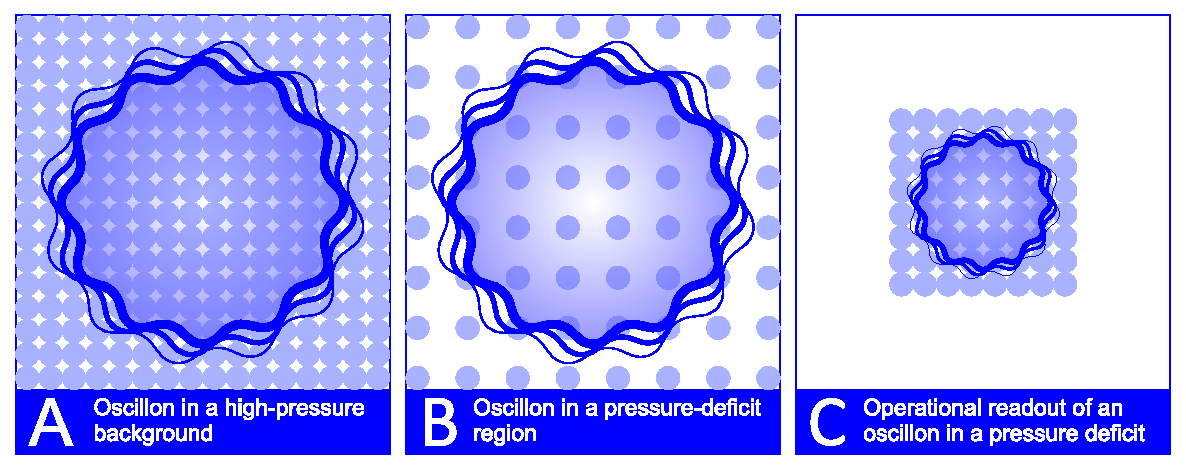
\includegraphics[width=\textwidth]{figures/figure_3.pdf}
\caption{\textbf{Operational readout of an oscillon within a pressure-deficit zone.}
\textbf{(A)} In an unperturbed foundation-medium whose pressure is higher than in the deficit region, an oscillon occupies a comparatively dense nodal arrangement; inter-node coupling is stronger and local processes proceed at a higher coordinate rate.
\textbf{(B)} Within a pressure-deficit region, foundation nodes are rarefied; operational inter-node separation increases, the transmission rate falls, and local clocks run more slowly in external coordinate time.
\textbf{(C)} In external readout, an oscillon within a pressure deficit has a slower clock rate, smaller operational size, and altered effective mass; the larger internal gaps are not directly measurable.}
\label{fig:figure_3_v2}
\end{figure}

\subsection{The Quadratic Relation and the Factor of Two}

The quadratic relation arises from two coordinate readouts of the same local standard. Both the coordinate length of a local ruler and its clock rate scale with $p$. The clock's coordinate period therefore scales as $p^{-1}$, so the coordinate speed of light, defined by the ratio of a ruler interval to a clock period, scales as $p/(p^{-1})=p^2$.

Writing the dimensionless pressure factor as $p$, the biconformal scaling law is
\begin{equation}
\frac{L_{\rm coord}}{L_0} = \frac{m_{\rm eff}}{m_0} = \frac{\Omega_t}{\Omega_{t,0}} = p, \qquad \frac{c_{\rm coord}}{c_0} = p^2, \qquad p = e^{\varphi/2}.
\end{equation}

Here $L_{\rm coord}$ is the length assigned to a local ruler in the distant asymptotic coordinate chart. In its own environment, the ruler still defines one unchanged local unit. The clock law gives $d\tau=p\,dt$, while ruler calibration gives $d\ell=p^{-1}d\sigma$. The temporal metric coefficient is therefore $p^2$ and the spatial coefficient is $p^{-2}$. A null signal has coordinate speed $p^2c_0$; measuring it with the same local ruler and clock gives the invariant local speed $c_0$.

A similar power-law dependence appears in the polarizable-vacuum (PV) models of Robert Dicke and Harold Puthoff \citep{dicke1957,puthoff2002}. $\RefG$ relates these exponents to the fundamental ontological distinction between nodes and their connecting links.

The externally determined effective mass of a single oscillon depends on the foundation's pressure-deficit profile through the exponential factor $e^{\varphi/2}$:
\begin{equation}
m_{\rm eff} = m_0 e^{\varphi/2}.
\end{equation}

On the deficit branch, $\varphi < 0$, so the pressure factor lies in the interval $0 < p < 1$. This relation describes the local external readout of an individual oscillon in a specified inhomogeneous background: as the deficit in $\varphi$ deepens, its operational size and $m_{\rm eff}$ decrease. The total gravitational charge of the extended system generating the deficit is determined separately by volume integration. This relation follows from the theory's first-order biconformal branch.

Four distinct physical quantities enter this description:
\begin{enumerate}[label=\arabic*.]
\item \textbf{Oscillon internal state and proper energy} ($M_{\rm proper}$);
\item \textbf{Single-oscillon effective refractive mass in a given background} ($m_{\rm eff}$);
\item \textbf{Active source profile of the induced pressure deficit} ($M_{\rm active}$);
\item \textbf{Total asymptotic gravitational charge of the system} (ADM/Komar mass: \citealt{arnowitt1962,komar1959}).
\end{enumerate}

These four quantities define two levels of accounting. The first separates the oscillon's internal energy from its externally determined contribution in a given environment. The second separates the active core and medium contributions to the externally determined mass. At the asymptotic boundary, these contributions form a single charge, with each deficit contribution counted once.

An oscillon is a localized resonant structure of the common foundation. Its resonant influence extends beyond the localized structure into the surrounding medium. The overlapping influence of many oscillons encompasses the foundation-medium and lowers its background pressure. $\RefG$ associates this collective process with spatial relaxation.

As the region affected by the resonant interaction expands, local pressure, externally determined mass, operational size, coordinate clock rate, and coordinate light speed change together. Falling pressure and decreasing $p$ weaken subsequent resonant coupling, slowing relaxation through negative feedback. On a homogeneous background, this process approaches the fully relaxed limit asymptotically.

The corresponding biconformal metric expresses the $p/p^2$ scaling as
\begin{equation}
ds^2 = e^\varphi c^2 dt^2 - e^{-\varphi} d\boldsymbol{\sigma}^2, \qquad \varphi = -\frac{2U}{c^2},
\end{equation}
where $U>0$ is the gravitational potential of the selected exponential branch and coincides at leading order with the magnitude of the Newtonian potential. In the weak-field limit ($U/c^2 \ll 1$), the metric components expand in a Taylor series:
\begin{equation}
g_{00} = e^\varphi \approx 1 - \frac{2U}{c^2} + \frac{2U^2}{c^4} + \cdots, \qquad g_{ij} = -e^{-\varphi}\delta_{ij} \approx -\left(1 + \frac{2U}{c^2} + \cdots\right)\delta_{ij}.
\end{equation}

On the selected common-scaling branch, the shared clock--ruler relations determine the biconformal metric and its first-order spatial response. A static functional determines the weak-field source profile under three conditions: the response is additive and logarithmic, $u=-\ln p$; the gradient term is canonical; and the coupling to the active source density entering Gauss's law is linear. Variation of this functional, together with the asymptotic boundary condition and Gauss charge, gives $u=GM/(c^2r)$.

In this static, spherically symmetric weak-field description, the first post-Newtonian (1PN) metric expansion yields the Parameterized Post-Newtonian (PPN) coefficients:
\begin{equation}
\beta = 1, \qquad \gamma = 1.
\end{equation}

Here $\gamma=1$ is the first-order geometric consequence of the common clock--ruler response. The logarithmic static response supplies the second-order temporal coefficient $\beta=1$.

\paragraph{Covariant Medium and an Exact Static Exterior.}

The exponential clock--ruler geometry admits an explicit covariant medium realization \citep{lotishvili2026medium}. In units $c=\hbar=1$ and signature $(+---)$, the medium is described by a clock scalar $\Phi$, three material labels $\phi^A$, and a dimensionless deficit-response field $H$. The labels describe material deformation, the clock defines a local temporal direction and spatial projector, and the response field reciprocally rescales the clock and deformation invariants. These quantities are defined by
\begin{equation}
\begin{aligned}
Y&=g^{\mu\nu}\nabla_\mu\Phi\nabla_\nu\Phi,
&u_\mu&=\frac{\nabla_\mu\Phi}{\sqrt Y},\\
\gamma^{\mu\nu}&=u^\mu u^\nu-g^{\mu\nu},
&B^{AB}&=-g^{\mu\nu}\nabla_\mu\phi^A\nabla_\nu\phi^B,\\
\widehat Y&=e^{-2H}Y,
&\widehat B^{AB}&=e^{2H}B^{AB}.
\end{aligned}
\end{equation}
The physical domain has $Y>0$ and positive-definite $B^{AB}$. The three deformation invariants are $\widehat I_1=\operatorname{Tr}\widehat B$, $\widehat I_2=[(\operatorname{Tr}\widehat B)^2-\operatorname{Tr}(\widehat B^2)]/2$, and $\widehat I_3=\det\widehat B$. This is the covariant language of self-gravitating media \citep{ballesteros2016medium}. The specified classical action is
\begin{equation}
\begin{aligned}
S={}&\int d^4x\sqrt{-g}\left[\frac{M_{\rm Pl}^2}{2}R+\mathcal L_{\rm med}\right]+S_{\rm m}[g,\psi],\\
\mathcal L_{\rm med}={}&-M_*^4F(\widehat Y,\widehat I_1,\widehat I_2,\widehat I_3)
-\omega_HM_{\rm Pl}^2\gamma^{\mu\nu}\nabla_\mu H\nabla_\nu H,
\end{aligned}
\label{eq:medium_action}
\end{equation}
where $M_{\rm Pl}^{-2}=8\pi G$, $M_*>0$ is a response scale, and ordinary matter $\psi$ couples universally and minimally to the same metric. The projected-gradient coefficient is dimensionless. This gradient acts within the spatial slice orthogonal to the clock direction and contributes to the gravitational source through its metric variation. The material labels $\phi^A$ describe the continuum medium, whereas the oscillon's complex wave field belongs to the matter sector. Here $H$ denotes the medium-response field, distinct from the cosmological Hubble function.

At the quiescent normalized state $\widehat Y=1$, $\widehat B^{AB}=\delta^{AB}$, choose $F=F_{,\widehat Y}=F_{,\widehat B^{AB}}=0$. With $\omega_H=1$, the ordinary-matter-free exterior then has the exact solution
\begin{equation}
\begin{gathered}
ds^2=e^{-2m/r}dt^2-e^{2m/r}(dr^2+r^2d\Omega^2),\\
\Phi=t,\qquad \phi^A=x^A,\qquad H=\frac{m}{r},\qquad r\ge r_c>0.
\end{gathered}
\label{eq:medium_exterior}
\end{equation}
All exterior metric and medium field equations are satisfied. The response function contributes no source on this background; the projected $H$ gradient supplies the entire exterior stress--energy tensor:
\begin{equation}
\frac{\Theta^\mu{}_{\nu}}{M_{\rm Pl}^2}
=\frac{m^2e^{-2m/r}}{r^4}\operatorname{diag}(-1,1,-1,-1).
\end{equation}
The normalized flux $Q_H=-r^2H'=m$ is fixed by boundary data and conserved, and the asymptotic geometry gives $m=GM_{\rm ADM}$. On this exact exterior branch, $p=e^{-H}$ and $\varphi=-2H$: the clock rate and coordinate ruler length scale with $p$, while the coordinate speed of light scales with $p^2$. The intuitive scaling law is thus realized by an exact exterior solution of a specified action. The relation between $H$ and the foundation pressure $P_F$ is a constitutive question.

The exponential geometry has a history beginning with Papapetrou \citep{papapetrou1954,boonserm2018exponential}; the result here is its exact embedding in the specified clock--label--response action. Its static expansion gives the coefficients $\beta=\gamma=1$. At the next spatial order, $e^{2m/r}=1+2m/r+2m^2/r^2+\cdots$, whose quadratic coefficient is $2$ compared with Schwarzschild's $3/2$ in isotropic coordinates.

\paragraph{Relational Coframe, Einstein--Hilbert Geometry, and Full 1PN.}

The covariant equations in this subsection use the $(-+++)$ signature; the preceding biconformal presentation uses $(+---)$.

The static $p$ profile represents the volumetric scalar projection of the full geometry. The complete local geometry is described by a \textbf{relational coframe} $e^A{}_\mu$: a system of local frame one-forms encoding volume, shape, shear, orientation, and temporal direction. The coframe defines a single operational metric,
\begin{equation}
g_{\mu\nu}=\eta_{AB}e^A{}_\mu e^B{}_\nu.
\end{equation}
The spacetime orientation of the coframe and the oscillon's internal three-axis structure are physically distinct; color is associated with the latter in the particle map. Neighboring coframes are compared through a flat, metric-compatible inertial connection, while the electromagnetic channel has its own $U(1)$ connection. The failure of an infinitesimal parallelogram to close under coframe transport is \textbf{geometric torsion}---the measure of non-integrable deformation in the coframe continuum.

The leading low-energy class of the post-Genesis relational-coframe continuum is defined by three conditions:
\begin{enumerate}[label=\arabic*.]
\item The action is local, reversible, constant-coefficient, parity-even, and quadratic in torsion.
\item The phase sector is minimally coupled, with no unsuppressed mixed operator contributing at the same order.
\item The linear Minkowski limit is regular, while coframe orientation remains an inertial gauge freedom and does not generate an independent long-range physical orientation mode.
\end{enumerate}
Within this class, the unique coefficient ratio gives the TEGR combination. The three independent quadratic torsion invariants are
\begin{equation}
I_1=T^\rho{}_{\mu\nu}T_\rho{}^{\mu\nu},\qquad
I_2=T^\rho{}_{\mu\nu}T^{\nu\mu}{}_\rho,\qquad
I_3=T_\mu T^\mu,\quad T_\mu=T^\nu{}_{\nu\mu}.
\end{equation}
Their TEGR combination is
\begin{equation}
T_{\rm TEGR}=\frac14 I_1+\frac12 I_2-I_3.
\end{equation}
The selected low-energy action is therefore
\begin{equation}
S_F=-\frac{c_0^3}{16\pi G}\int d^4x\,e
\left(T_{\rm TEGR}+2\Lambda_F\right)
+S_C[g,J,\theta_C]+S_{\partial},
\end{equation}
where $S_C$ is the covariant phase-current action and $S_{\partial}$ is the matched boundary functional. The minus sign of the gravitational torsion term combines with the following torsion--curvature identity to recover the Einstein--Hilbert sign exactly.
With the $(-+++)$ signature, the exact connection identity
\begin{equation}
R_{\rm LC}=-T_{\rm TEGR}+\frac{2}{e}\partial_\mu(eT^\mu),
\end{equation}
converts the coframe action to the Einstein--Hilbert action up to a boundary term \citep{jimenez2020ngr,maluf2013tegr}. Here $R_{\rm LC}$ is the Ricci scalar of the Levi--Civita connection, $e=\det(e^A{}_\mu)$ is the coframe determinant, and $T^\mu$ is the torsion trace. The actions are exactly equivalent for compactly supported variations with suitable asymptotic falloff, or with an exactly matched boundary functional. Under these conditions, Einstein geometry is the continuum form of relational-coframe dynamics. The Fierz--Pauli/Deser spin-2 self-coupling construction independently checks the same final operator.

$S_C$ describes a barotropic, isentropic, irrotational phase current with a single potential on its positive, stable, causal constitutive branch: $\rho_C>0$, $\rho_C'>0$, and $0\le n_{C,{\rm op}}\rho_C''(n_{C,{\rm op}})/\rho_C'(n_{C,{\rm op}})\le1$. Variation with respect to $\theta_C$ gives the conserved current, whereas metric variation gives the Hilbert stress--energy tensor \citep{brown1993fluid}
\begin{equation}
T^C_{\mu\nu}=(\rho_C+p_C)u_\mu u_\nu+p_Cg_{\mu\nu}.
\end{equation}
Here $n_{C,{\rm op}}$ is the phase-charge density per operational volume and $p_C=n_{C,{\rm op}}\rho_C'(n_{C,{\rm op}})-\rho_C(n_{C,{\rm op}})$ is the thermodynamic pressure of the phase sector, whereas $P_F$ is the operational readout of the foundation's background pressure. These are distinct physical variables whose constitutive relation must be determined by foundation microphysics. When the source is restricted to the phase-current sector, the field equation is
\begin{equation}
G_{\mu\nu}+\Lambda_Fg_{\mu\nu}
=\frac{8\pi G}{c_0^4}T^C_{\mu\nu}.
\end{equation}
For the general case, the right-hand side contains $T^{\rm tot}_{\mu\nu}$; every physical stress--energy sector in the action enters that total once through its own metric variation.

The selected TEGR-equivalent coframe action places $\RefG$ and General Relativity in the same 1PN equivalence class under five conditions:
\begin{enumerate}[label=\arabic*.]
\item Through 1PN order, the complete action consists of the Einstein--Hilbert operator and the matter action.
\item Matter couples universally and minimally to the same metric.
\item The source is recorded by one complete, conserved stress--energy tensor.
\item $\RefG$ and GR use the same local source, PPN gauge, background, and boundary conditions.
\item No additional unsuppressed field or operator participates in the 1PN degree-of-freedom inventory.
\end{enumerate}
Under these conditions, the complete standard PPN vector is
\begin{equation}
\gamma=\beta=1,\qquad
\xi=\alpha_1=\alpha_2=\alpha_3=
\zeta_1=\zeta_2=\zeta_3=\zeta_4=0.
\end{equation}
The result applies to isolated, weak-field, slowly moving, weakly self-gravitating sources. The static, spherically symmetric calculation provides an independent local check: $\gamma=1$ follows from the common clock--ruler response, while $\beta=1$ follows from the logarithmic law $u=-\ln p$.

For a light-clock realization, the coordinate period is the operational length divided by the coordinate speed of light ($\Delta t \sim L_{\rm oper}/c_{\rm coord}$). Here the operational length is the ruler's coordinate footprint. If a pressure drop halves this length ($p = 1/2$) while reducing coordinate light speed by a factor of four ($p^2 = 1/4$), the period doubles and the clock runs at half its previous coordinate rate.

In the shared static, spherically symmetric regime, the 1PN effects controlled by $\beta=\gamma=1$ recover the classical predictions of General Relativity: the gravitational deflection of light, Shapiro time delay, gravitational redshift, and planetary perihelion precession \citep{bertotti2003,will2014}. In particular, the Cassini radio-link experiment measured $\gamma-1=(2.1\pm2.3)\times10^{-5}$.

Historically, including the spatial metric component $g_{ij}$ supplied the \textbf{factor of two} between Einstein's 1911 half-deflection prediction and the full geometric result of 1915--1916 \citep{einstein1916,shapiro1964}. In $\RefG$, this factor follows from two coordinate readouts of the same local standard: material size and clock rate scale with $p$, while the coordinate speed of light reconstructed from them scales with $p^2$.

\subsection{Refractive Attraction, Inertia, and the Absence of Friction}

An oscillon is an extended wave structure propagating through spatial gradients of foundation-medium pressure and coordinate wave speed. Its phase velocity is higher on the denser side and lower on the rarefied, pressure-deficit side. According to the Huygens--Fresnel principle and the eikonal equation, the wavefront therefore bends toward lower pressure and lower coordinate speed: it undergoes \textbf{refraction}. In the static weak-field limit, the pressure deficit generated by a massive body defines an effective optical-geometric medium. The refracted trajectory of a matter wave packet in this medium manifests macroscopically as gravitational attraction.

In $\RefG$, a body's free fall in the Earth's field is associated with the refractive deflection of the oscillon structures constituting its atoms. The deflection is directed toward the lower-pressure region with slower coordinate propagation produced by the Earth. In this description, gravitational attraction is the local response of wave-like matter to an inhomogeneous medium.

In the relational-coframe description, the pressure deficit and non-integrable deformation characterize the gravitational geometry. The scalar $p$ profile determines the common volumetric response of clocks, rulers, and wave propagation, while the coframe describes the full tensor structure. In the post-Genesis continuum, the TEGR action equals the Einstein--Hilbert action up to a boundary term; metric variation of the phase-current sector yields the Hilbert source $T^C_{\mu\nu}$ on the right-hand side of the field equation. Every physical stress--energy contribution in the action enters the total Hilbert tensor once. A gravitational potential well is a region of reduced pressure and altered geometry, where the total mass of a bound system is smaller than the sum of its free constituents by the mass equivalent of the binding energy ($\Delta M=B/c^2$).

GW150914 provides an observational example of this energy balance: the difference between the externally determined initial binary mass and final remnant mass, equivalent to roughly three solar masses ($3\,M_\odot$), was radiated as gravitational-wave energy \citep{abbott2016}. In the $\RefG$ description, two oscillatory sources reorganize into a single, deeper deficit profile. In the TEGR-equivalent low-energy geometry, the rapid nonlinear change is described by the standard transverse-traceless tensor wave.

$\RefG$ associates \textbf{inertia} with the dynamic deformation of an oscillon's deficit profile during acceleration. An externally accelerated oscillon develops an asymmetric pressure profile along the direction of motion. The resulting gradient asymmetry produces a response from the medium opposing the acceleration: the inertial force. During deceleration, the orientation of the pressure-profile asymmetry reverses.

On a Lorentz-covariant, localized finite-energy branch satisfying the Laue condition ($\int T^{ij}\,d^3x=0$ for all $i,j$), the system's total Noether energy determines the inertial coefficient \citep{noether1918,laue1911}. Including the same energy as the universal gravitational source gives $m_i = m_g$ at leading order. The French MICROSCOPE satellite mission tests this universality at the $10^{-15}$ level \citep{touboul2022}.

On the branch of uniform, rectilinear motion, the oscillon's wave structure is transmitted symmetrically between foundation nodes without energy loss. $\RefG$ associates \textbf{frictionless inertial motion} with this regime of coherent phase transfer: the oscillon moves through the nodal medium by successive transmission of its wave state. In the low-energy continuum description, the common Lorentzian cone relates the limiting speed of phase transmission to the metric light cone.

\subsection{Local Unobservability and the Principle of Relativity}

A local observer in a gravitational field measures an unchanged local clock rate and spatial scale because the observer's clock, ruler, and body are made from the same foundation-medium. A pressure change rescales the entire local system by a common factor. Changes that are slow relative to internal periods are adiabatic: they preserve the oscillatory mode and induce no quantum transitions. On this common-scaling branch, dimensionless ratios are exactly invariant when both components undergo the same adiabatic rescaling; $\RefG$ places the fine-structure constant $\alpha$ in this class.

Two classes of experiment constrain this description:
\begin{itemize}
\item \textbf{Gravitational Redshift:} The Pound--Rebka experiment \citep{pound1960}, the Gravity Probe A hydrogen-maser experiment \citep{vessot1980}, and the Galileo satellite tests \citep{delva2018,herrmann2018} measure the dependence of clock rate on gravitational potential with high precision. $\RefG$ interprets this dependence as the temporal component of the common pressure--geometric response.
\item \textbf{Invariance of Dimensionless Ratios:} Absorption spectra of distant quasars and laboratory optical atomic clocks constrain possible cosmological variation of $\alpha$ to $|\Delta\alpha/\alpha| \lesssim 10^{-6}$ \citep{kotus2017}. This observational bound provides a test consistent with the $\RefG$ prediction of self-calibration through a common clock rate.
\end{itemize}

The null result of the Michelson--Morley experiment corresponds to the medium's \textbf{common-mode self-calibration}, whereas gravitational-wave detections by LIGO, Virgo, and KAGRA measure a \textbf{differential tensor response}:
\begin{itemize}
\item When the foundation-medium changes uniformly and isotropically throughout a local region, rulers, clocks, and light propagation rescale together, making local measurements self-calibrating. Modern optical cavities constrain directional anisotropy in the speed of light at the level $\Delta c/c \lesssim 10^{-17}$ (\citealt{herrmann2009}).
\item A gravitational wave is a time-dependent, quadrupolar differential strain ($h_+, h_\times$): it stretches space along one transverse axis while compressing it along the perpendicular axis. These opposite-sign deformations prevent common-mode cancellation and produce a measurable phase shift between the interferometer arms.
\end{itemize}

FitzGerald--Lorentz length contraction \citep{fitzgerald1889,lorentz1892} is a historical antecedent of this reasoning. $\RefG$ relates the contraction to the fact that measuring instruments are themselves wave excitations of the foundation-medium.

In the TEGR-equivalent low-energy geometry, tensor waves propagate on the common metric light cone, so $v_{\rm gw}=c$ at this order. The nearly simultaneous detection of gravitational waves and gamma rays from the binary neutron-star merger GW170817 constrains their fractional speed difference \citep{abbott2017}:
\begin{equation}
-3 \times 10^{-15} \le \frac{v_{\rm gw} - c}{c} \le +7 \times 10^{-16}
\end{equation}
The orbital decay of relativistic binary pulsars (PSR B1913+16, PSR J0737-3039A/B) confirms the general-relativistic normalization of quadrupole energy loss to an accuracy of $10^{-3}$--$10^{-4}$ \citep{weisberg2016,kramer2021}. The LIGO--Virgo--KAGRA GWTC-3 catalogue also places stringent limits on the scalar breathing-polarization contribution \citep{ligovirgokagra2022}.

With metric signature $(-+++)$, an operational invariant of this description is the difference between the proper times accumulated by two clocks along worldlines with different gravitational and kinematic histories:
\begin{equation}
\tau_a=\frac{1}{c}\int_{\gamma_a}\sqrt{-g_{\mu\nu}dx^\mu dx^\nu},
\qquad
\Delta\tau=\tau_1-\tau_2.
\end{equation}

The accumulated proper times are invariant records of the clocks' trajectories through different pressure regimes. Locally measured instantaneous rates and lengths are relative properties of the common medium.

\subsection{Historical Context and the Role of RefG}

Refractive descriptions of gravity in terms of an optical medium date to the development of general relativity. In 1911--1912, before its final geometric formulation, Albert Einstein related the coordinate speed of light to the gravitational potential \citep{einstein1911,einstein1912}:
\begin{equation}
c(\Phi) = c_0 \left(1 + \frac{\Phi}{c^2}\right)
\end{equation}
The optical properties of moving media had been studied earlier. In 1851, Armand Hippolyte Fizeau demonstrated partial light dragging in moving water, described by Fresnel's dragging coefficient (\citealt{fizeau1851}). In 1923, Walter Gordon showed that electromagnetic waves in a moving dielectric medium follow the null geodesics of an effective Lorentzian (pseudo-Riemannian) metric \citep{gordon1923}. This established the first rigorous mathematical connection between medium optics and spacetime geometry.

In 1957, Robert Dicke described gravitation through a variable vacuum refractive index \citep{dicke1957}. William Unruh's 1981 work established the basis of modern \textbf{analogue gravity}: acoustic waves in a moving fluid with a supersonic region propagate according to an effective metric with an acoustic black-hole horizon \citep{unruh1981}.

Grigory Volovik's condensed-matter program \citep{volovik2003} and the review by Barceló, Liberati, and Visser \citep{barcelo2011} showed how local Lorentz invariance and effective curved spacetime can emerge from the microscopic dynamics of background quantum condensates, including those in liquid helium-3 and helium-4. In 2019, Jeff Steinhauer's group experimentally observed the acoustic analogue of quantum thermal Hawking radiation in a rubidium Bose--Einstein condensate \citep{munozdenova2019}.

Related research explores the \textbf{thermodynamic and entropic origins} of gravity:
\begin{itemize}
\item Andrei Sakharov interpreted gravity as an elastic vacuum phenomenon induced by quantum fluctuations \citep{sakharov1967};
\item Ted Jacobson demonstrated that Einstein's field equations arise directly as an equation of state from the thermodynamic entropy balance ($\delta Q = T dS$) across local Rindler horizons \citep{jacobson1995};
\item Erik Verlinde described gravitational attraction as an entropic effect driven by changes in information on holographic screens \citep{verlinde2011}.
\end{itemize}

These approaches and $\RefG$ share the view that spacetime geometry is a derived physical structure. $\RefG$ takes a pressure--refractive foundation-medium as its physical source.

Refractive Gravity ($\RefG$) brings together four principles related to these approaches:
\begin{enumerate}[label=\arabic*.]
\item \textbf{Monistic Ontological Unity:} The foundation-medium produces both the geometric response and the oscillon structures constituting matter, measuring instruments, and the observer. The hydrodynamic interpretation is thereby incorporated into a single calculable physical framework.
\item \textbf{Population-Locked Local Frequency Scale ($\Omega_t$):} Nonlinear synchronization provides a specific mechanism for local self-calibration. For a physical oscillon, it predicts a spectrum in which all stable-mode frequencies scale with the common pressure factor while their dimensionless ratios remain unchanged.
\item \textbf{One Foundation with a Multicomponent Geometric Response:} Pressure and expansion govern the scalar readout, symmetric deformation and shear determine the tensor response, and orientation remains an inertial gauge freedom. These components define one operational geometry. Each physical stress--energy contribution in the action couples to its metric once.
\item \textbf{From Relational Coframe to Einstein--Hilbert:} In the post-Genesis coframe's leading local, reversible, constant-coefficient, parity-even quadratic-torsion class, with minimal phase coupling and no unsuppressed mixed operator at that order, the regular linear Minkowski limit determines the TEGR coefficient ratios by requiring the absence of an independent physical orientation mode. The exact torsion--curvature identity converts the action to Einstein--Hilbert form up to a boundary term \citep{jimenez2020ngr,maluf2013tegr}. The Fierz--Pauli linear spin-2 construction and Deser's universal self-coupling provide a separate route to the same final operator. In four dimensions, Lovelock's theorem gives the corresponding uniqueness statement for local metric field equations of at most second differential order, up to normalization and a cosmological term \citep{deser1970,lovelock1971}.
\end{enumerate}

$\RefG$ combines optical refraction, topological solitons, and thermodynamic balance within one research program. Each connection is subject to its corresponding mathematical and observational tests.

\section{Three Scales and Cosmological Horizons}

\subsection{The Local Scale: Compact Objects, Internal State, and External Readout}

The pressure mechanism described in the preceding chapters is considered at three distinct scales:
\begin{enumerate}[label=\arabic*.]
\item \textbf{Local scale:} the localized pressure-deficit profile surrounding oscillons and compact relativistic bodies;
\item \textbf{Galactic scale:} the coherent vortical flow of the foundation;
\item \textbf{Cosmological scale:} relaxation of the background pressure driven by geometric expansion of the foundation-medium, together with the relation between coordinate and process time.
\end{enumerate}

These are three dynamical regimes of one foundation. The local regime describes spatially inhomogeneous pressure-deficit profiles, the galactic regime describes the coherent long-range response, and the cosmological regime describes the global evolution of the foundation.

In an extreme gravitational regime, an object's \textbf{internal state} ($M_{\rm proper}$) and its \textbf{externally inferred active gravitational mass} ($M_{\rm external}$) are distinct quantities. The compact-object map of $\RefG$ distinguishes the conserved internal content of accumulated matter from the gravitational charge inferred at a distance. A remote observer measures the state through its pressure-deficit profile, clock rate, and changing operational size, while the interior geometry, horizon, and global causal structure are determined by the complete nonlinear field solution.

Two-channel accounting distinguishes the object's local internal state from its asymptotic gravitational readout. The internal channel describes the local state of matter, conserved charges, and proper scale; the external channel records the deficit profile, clock rate, operational size, and total mass inferred at a distance. Gravitational compression produces a pronounced difference between these readouts, which nevertheless describe the same physical object.

$\RefG$ relates the mass defect of a merging compact system to nonlinear changes in binding and in the deficit profile. Its quantitative connection to the outgoing tensor flux is determined by the complete dynamical solution, with the gravitational-wave event GW150914 providing the experimental benchmark \citep{abbott2016}.

The covariant medium action gives a concrete exterior for this picture, while a regular interior can be stated as an explicit geometric target \citep{lotishvili2026medium}. In units $c=1$ and signature $(+---)$, write
\begin{equation}
ds^2=B(r)\,dt^2-A(r)\bigl(dr^2+r^2d\Omega^2\bigr),
\qquad x=\frac{r}{r_c},\qquad q=\frac{2m}{r_c},\qquad 1<q<2.
\end{equation}
The exterior has $\ln A=q/x$ and $\ln B=-q/x$. The following interior, for $0\le x\le1$, joins it with two continuous derivatives:
\begin{equation}
\begin{aligned}
\ln A&=q\left(\frac{35}{8}x^2-\frac{21}{4}x^4+\frac{15}{8}x^6\right),\\
\ln B&=-q+q\left(-\frac{11}{8}x^2+\frac94x^4-\frac78x^6\right).
\end{aligned}
\label{eq:medium_core_target}
\end{equation}
At the center, $A(0)=1$, $B(0)=e^{-q}$, and both first derivatives vanish. The resulting $C^2$ geometry has a regular center, bounded curvature and effective stress--energy, and is geodesically complete. Its temporal metric coefficient is positive everywhere: this particular kinematic construction describes a horizonless compact object. The clock factor satisfies $\sqrt B>0.2876$ throughout the stated family, so the clock rate does not vanish at the center. The construction is a geometric benchmark for testing the strong-field source; its interior scale relation must be determined from a solution of the medium action.

The distinction between clock and ruler readouts is explicit. Relative to the asymptotic coordinate standards, let $p_t=\sqrt B$ be the static-clock factor and $p_L=A^{-1/2}$ the coordinate length of a fixed proper ruler. They coincide in the exterior, where $p_t=p_L=e^{-H}$, but in the core
\begin{equation}
AB=e^{q(x^2-1)^3},\qquad \frac{p_t}{p_L}=\sqrt{AB}.
\end{equation}
The local speed of light remains $c$ in both regions, while its radial coordinate speed in the asymptotically normalized coordinates is $p_t p_Lc$. The two interior readouts differ; the exterior one-factor scaling law does not extend to this particular core geometry.

In the static clock-adapted description, the medium also connects the interior and exterior through the $H$-field flux. A regular center and a junction without a surface source for $H$ require
\begin{equation}
Q_H(r)=-\sqrt{AB}\,r^2H'(r),\qquad Q_H(0)=0,\qquad Q_H(r_c)=m.
\end{equation}
The regular interior must generate this flux and the required stress--energy tensor from the same action. Equation~\eqref{eq:medium_core_target} supplies the geometric benchmark for that source-matching problem.

The exterior optical geometry is also determined exactly. Its unstable circular light orbit lies at the isotropic radius $r=2m$, with critical impact parameter
\begin{equation}
b_{\rm crit}=2em,
\end{equation}
which is $4.63\%$ larger than the Schwarzschild value $3\sqrt3\,m$ at the same ADM mass. For a transparent regular core, this is a critical scattering boundary: a ray entering the interior may re-emerge. The observed image depends on absorption, emission, radiative transfer through plasma, and rotation \citep{gralla2019rings}.

Assessing singularity avoidance requires the local source, curvature measured in freely falling frames, and geodesic extendibility. The effective source of the specified polynomial core violates the strong energy condition (SEC) near the center. Its effective energy density $\rho$ and radial pressure $P_r$ satisfy $\rho+P_r<0$ there, violating the null energy condition (NEC); the exact exponential exterior source likewise violates the radial NEC. These are properties of the named constructions. Penrose's null-convergence condition $R_{\mu\nu}k^\mu k^\nu\ge0$ is related to the NEC through Einstein's equation and must be considered together with the theorem's other global premises \citep{penrose1965}. A stable phase current satisfying $\rho_C+p_C>0$ remains an NEC-compatible source within its own action; the contribution of the additional medium source is determined by its separate variation.

Regular compact objects are an active subject of relativistic astrophysics. The Mazur--Mottola gravastar, for example, is a vacuum-condensate object without a singular point \citep{mazur2004}. Such alternatives may be distinguished from classical black holes by EHT shadow structure, quasinormal-mode spectra, and gravitational-wave echo limits \citep{eventhorizon2019,cardoso2019}. The compact-object picture of $\RefG$ is structurally related to this class and associates the internal state with the pressure--energy balance of the universal foundation.

\subsection{The Galactic Scale: Vortical Flow and MOND}

\paragraph{Observational Evidence.} In many disk galaxies, rotation curves at large radii do not follow the Keplerian decline expected from visible baryonic matter alone: their shapes vary, but they often flatten or decline more slowly than expected. Baryonic mass and asymptotic rotation speed obey a tight empirical relation---the baryonic Tully--Fisher relation ($M_b \propto v_f^4$; \citealt{tully1977,lelli2016}). An early result in this observational program was Vera Rubin and Kent Ford's measurement of Andromeda's rotation curve \citep{rubin1970}. In the \textbf{radial acceleration relation (RAR)}, 2,693 radial data points from 153 galaxies follow a single universal curve \citep{mcgaugh2016}.

The standard $\Lambda$CDM model accounts for these observations through approximately spheroidal cold-dark-matter halos. Modified Newtonian Dynamics (MOND), by contrast, introduces a universal acceleration threshold:
\begin{equation}
a_0 \approx 1.2 \times 10^{-10} \text{ m/s}^2,
\end{equation}
below which gravitational acceleration transitions from Newtonian $a_N$ to the deep-MOND regime $\sqrt{a_N a_0}$ \citep{milgrom1983}. Relativistic completions (such as TeVeS and Skordis--Złośnik models) incorporate additional dynamical vector and scalar fields \citep{bekenstein2004,skordis2021}.

\paragraph{The RefG Vortical Mechanism and Foundation-Medium Polarization.} At galactic scales, $\RefG$ relates the additional deficit to large-scale \textbf{vortical flow and induced polarization} of the foundation-medium. An ordered rotational regime deepens the central pressure deficit, while baryonic oscillons and the surrounding flow form one shared refractive profile.

At the macroscopic level, this response is described by a Ginzburg--Landau-type local effective potential:
\begin{equation}
W(g_v, g_N) = \frac{1}{3} g_v^3 + \frac{1}{2} g_N g_v^2 - a_0 g_N g_v,
\end{equation}
where $g_v$ is the foundation-medium response field, $g_N$ is the baryonic Newtonian acceleration, and $a_0 \approx 1.2 \times 10^{-10}\text{ m/s}^2$ is the universal transition acceleration scale. The variational equilibrium condition, $\partial W / \partial g_v = 0$, yields:
\begin{equation}
g \equiv g_N + g_v, \qquad g_N = \frac{g^2}{g + a_0}.
\end{equation}

In the deep asymptotic regime ($g \ll a_0$), this relation approaches $g^2 \simeq a_0 g_N$, yielding for circular orbits the Baryonic Tully--Fisher Relation ($v^4 = G M_b a_0$) without individual galaxy tuning parameters.

\paragraph{Observational Check on SPARC Data.} Distinct from the published 153-galaxy, 2,693-point RAR sample, the cuts $\Delta V/V<10\%$ and $V_{\rm obs}>20\text{ km/s}$ select 2,788 points from 163 SPARC galaxies. With fixed $a_0$ and fixed mass-to-light ratios ($\Upsilon_{\rm disk}=0.5$, $\Upsilon_{\rm bulge}=0.7$), and without galaxy-by-galaxy parameter fitting, this comparison gives an RMS scatter of $0.141\text{ dex}$ and a mean residual of $-0.012\text{ dex}$ (Figure~\ref{fig:sparc_rar}).

\begin{figure}[htbp]
\centering
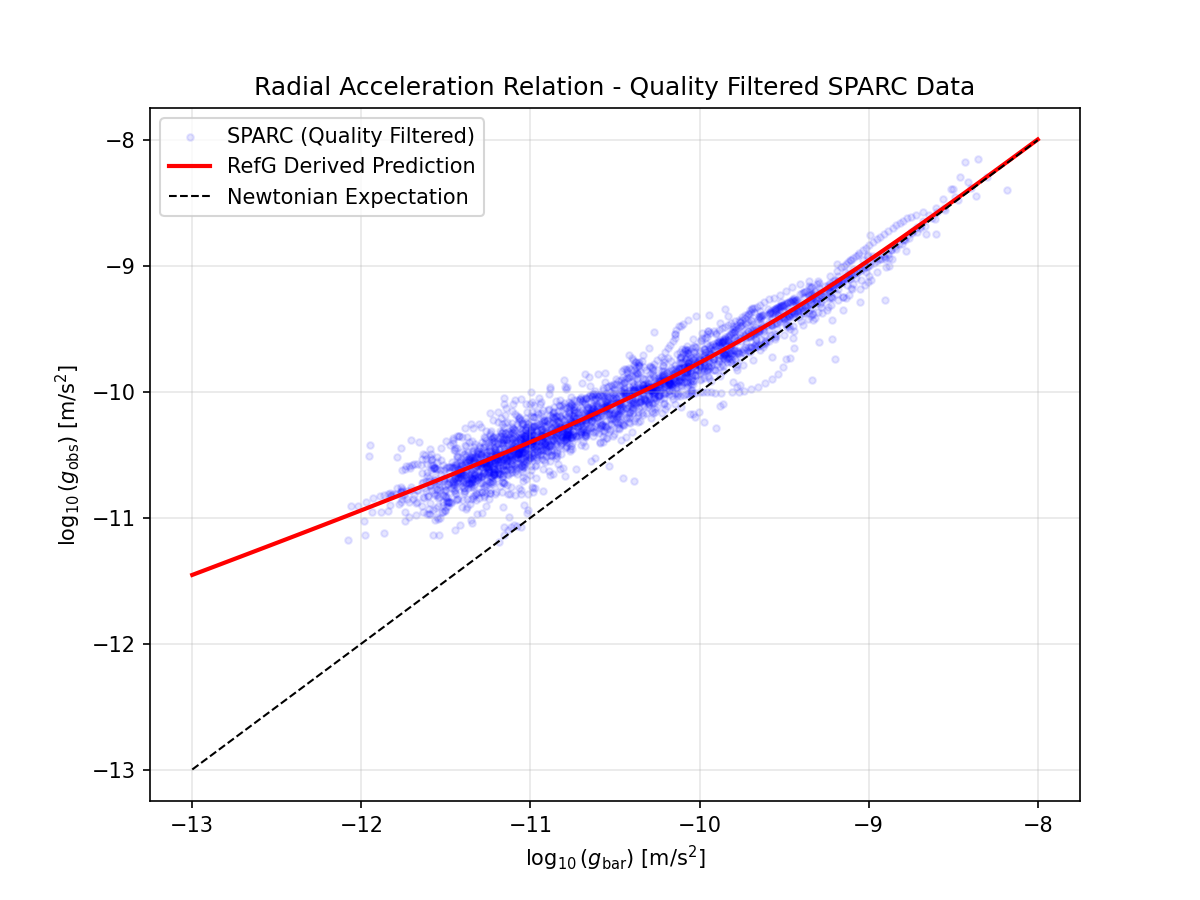
\includegraphics[width=0.85\textwidth]{figures/sparc_rar_real_validation.png}
\caption{\textbf{Radial Acceleration Relation comparison with SPARC data.} The observed radial acceleration $g_{\rm obs}=V_{\rm obs}^2/R$ versus the baryonic acceleration $g_{\rm bar}$ for 2,788 selected points across 163 disk galaxies. With fixed $a_0$ and mass-to-light ratios, but no galaxy-specific fitting, the algebraic $\RefG$ curve obtained from $W(g_v,g_N)$ gives an RMS scatter of $0.141\text{ dex}$ and a mean residual of $-0.012\text{ dex}$.}
\label{fig:sparc_rar}
\end{figure}

\paragraph{Disk Geometry and QUMOND Numerical Test.} For a finite-thickness Miyamoto--Nagai disk, transverse gradients of the algebraic field generate a geometric curl correction. On a $300\times300$ grid with $a=3\text{ kpc}$ and $b=300\text{ pc}$, Biot--Savart reconstruction gives, in this finite-grid configuration, a maximum radial-acceleration correction of $9.23\%$ relative to the one-dimensional algebraic mapping over $a\le r\le5a$.

\paragraph{Refractive Gravitational Lensing.} Along the flat rotation curve branch, $\Phi_{\rm eff} = v_f^2 \ln(r/r_0)$ and $n(r) \approx 1 - 2\Phi_{\rm eff}/c^2$. Integrating the transverse refractive index gradient yields a deflection angle $\hat{\alpha} = 2\pi v_f^2 / c^2$, matching the prediction of General Relativity for a singular isothermal sphere. Rotation and lensing thus emerge as two readouts of a single effective potential.

The closest modern analogue is the \textbf{Superfluid Dark Matter} model of Berezhiani and Khoury, in which a MOND-like force arises from phonon excitations of a condensate \citep{berezhiani2015}. Both approaches draw on the collective response of a coherent medium. In the superfluid-dark-matter model that medium is the phase of an additional particle component; in $\RefG$, the vortical flow is a large-scale regime of the unified foundation-medium itself.

\paragraph{Morphology.} In $\RefG$, galactic morphology reflects the flow regime of the foundation: ordered laminar rotation is associated with disk and spiral structure, whereas more chaotic or isotropic flow is associated with dispersion-supported elliptical galaxies.

\paragraph{Galaxy Clusters.} A simple modification of the acceleration law is often insufficient to account for the dynamical mass deficit in galaxy clusters, a problem first identified by Fritz Zwicky in observations of the Coma cluster \citep{zwicky1933}. $\RefG$ describes the cluster mass budget through three distinct channels:
\begin{enumerate}[label=\arabic*.]
\item The global nodal deficit of the long-wavelength resonant network;
\item Individual galaxies and the long-range pressure-deficit fields of their constituent oscillons;
\item Cluster-scale vortical circulation and the hydrodynamic memory of past mergers.
\end{enumerate}
All three enter a unified pressure-deficit budget, each counted exactly once.

Two decisive observational signatures distinguish this framework:
\begin{enumerate}[label=\arabic*.]
\item \textbf{Quantized Circulation:} If the foundation flow possesses a single-valued condensate phase, circulation is quantized in units of:
\begin{equation}
\Gamma = \oint \mathbf{v} \cdot d\mathbf{l} = n \frac{h}{m},
\end{equation}
where $m$ is the effective mass of the flow mode. For ultralight modes ($m \sim 10^{-22}\text{ eV}$), vortex filaments could be detected via weak lensing or stellar disk kinematics \citep{hu2000,hui2021}.
\item \textbf{Long-Lived Vortical Memory in the Bullet Cluster:} In the Bullet Cluster (1E 0657-558), weak-lensing centroids are displaced from the hot X-ray gas at $8\sigma$ significance and follow the collisionless galaxies \citep{clowe2006}. $\RefG$ associates this separation with the \textbf{persistence of vortical flow in the foundation-medium}: during the collision, hydrodynamic drag due to electromagnetic interactions slowed the gas, while the deficit profile continued moving with the galaxies for longer. The memory timescale, spatial profile, and lensing amplitude are components of a common dynamical description.
\end{enumerate}

The galactic mechanism is jointly testable against the SPARC/RAR relation \citep{lelli2016}, galaxy-cluster mass budgets, and Bullet-Cluster-type mergers. A combined test with the CMB, BAO, and large-scale-structure statistics will determine whether this galactic response and the cosmological neutral collective-phase source share one foundation-level normalization.

\subsection{The Cosmological Scale: Foundation Expansion and Its Internal Readout}

The cosmological history of $\RefG$ begins with the centerless, foundation-wide transition described in Section~1.2. It is the common origin of the first distinguishable relations. Distance and direction acquire physical meaning only after the first distinguishable connections have formed. In the centerless initial state, equivalent regions share this common initial boundary; a history ordered outward from a privileged site would break that initial symmetry. Local waves and oscillon centers arise only within the spatial layer that follows.

The sequence is: formation of the first relations, localization of oscillon seeds, overlap of their resonant fields, emergence of resonant coupling as the distinguishability threshold is crossed, growth of network connectivity, formation of stable oscillons, and long-term foundation expansion accompanied by pressure relaxation.

Four pressure variables carry distinct physical roles in this cosmological picture. The foundation background pressure $P_F$ is an operational readout that controls the common response factor $p$ of material scale and clock rate. The quantity $p_C=n_{C,{\rm op}}\rho_C'(n_{C,{\rm op}})-\rho_C(n_{C,{\rm op}})$ is the thermodynamic pressure of the neutral phase current. The ordinary thermal pressure is denoted by $P_{\rm th}$, while $P_*$ is the mechanical response of a homogeneous stationary vacuum phase.

The corresponding equations of state relate these four quantities. Keeping them distinct assigns every physical contribution of energy and pressure to its proper sector and prevents double counting. The geometric contribution $\Lambda_{\rm phase}$ of a constant phase density enters the total $\Lambda_{\rm eff}=\Lambda_{\rm bare}+\Lambda_{\rm phase}$ once. The initial thermal state is determined by the sectoral distribution of energy, the equation of state for $P_{\rm th}$, and energy exchange with radiation.

The observable physical content of the thermal state is encoded in dimensionless ratios, including
\begin{equation}
\Theta_\gamma=\frac{k_B T_\gamma}{E_{\rm atom}},
\qquad
\mathcal{R}_i=\frac{\Gamma_i}{H_A}.
\end{equation}
Here $E_{\rm atom}$ is the atomic energy scale, $\Gamma_i$ is the rate of the relevant microphysical process, and $H_A=(1/A)dA/d\tau$ is the expansion rate of the operational scale in process time. On the selected standard low-energy operational branch, the common $p$ scale is already encoded in the metric and does not re-enter these dimensionless ratios as a second factor; the observable content of temperature is determined by the actual energetic relation between matter and radiation. The CMB spectrum, recombination, and BBN provide a joint test of this thermodynamic map.

The quantity $R_{\rm act}(t)$ denotes a local post-origin activation or correlation scale within which nodal relations reach the minimum distinguishability threshold $\ell_*$. It is a local quantity; the homogeneous global geometry of the Universe is described by $A$. On a homogeneous background the same local rule applies around every node comoving with the network.

On the selected cosmological branch, formed matter follows the expanding nodal lattice of the foundation. For two galaxies comoving with the mean flow, let $N_{12}$ count the foundation nodes and links along the path defining their comoving separation. In the ideal expansion component, $N_{12}$ remains fixed while the physical length of each interval, $\ell_F(t)$, grows:
\begin{equation}
L_{12}(t)=N_{12}\,\ell_F(t).
\end{equation}
The constancy of $N_{12}$ applies specifically to the cosmological expansion component. Matter can move locally with respect to the lattice, rotate, collide, and undergo gravitational displacement; those processes can change $N_{12}$. In the selected ontological picture, growth of foundation separation in the mean Hubble flow is carried by the changing inter-node length scale.

The observer, the clock, and the ruler are made from the same foundation. The change in foundation scale is therefore read internally through the pressure response of the material standard. Define
\begin{equation}
a(t)=\frac{\ell_F(t)}{\ell_{F,0}},
\end{equation}
as the inter-node length scale of the foundation, and let $p(t)$ denote the material-standard scale. The causal chain of $\RefG$ is
\begin{equation}
a\uparrow
\;\longrightarrow\;
P_F\downarrow
\;\longrightarrow\;
p\downarrow.
\end{equation}
The operational ratio available to an internal observer is
\begin{equation}
A(t)=\frac{a(t)}{p(t)}.
\end{equation}
The ratio $A$ is the internal operational readout; $a$ and $p$ are not measured directly and separately. The internal activation scale $R_{\rm act}(t)$, the foundation length scale $a(t)$, and the material standard $p(t)$ are three distinct quantities. The first describes the local spread of stably distinguishable relations, the second the change in foundation inter-node length, and the third the pressure response of material size and clock rate.

\paragraph{Neutral Collective Phase and the Relaxation Law.}

A concrete post-Genesis realization of the relaxation law describes the organized foundation state by a neutral collective phase. In the foundation-volume representation,
\begin{equation}
\Psi_C=\sqrt{n_{C,F}}\,e^{i\theta_C}.
\end{equation}
Here $n_{C,F}$ is the organized collective phase-charge density per foundation volume, while $\theta_C$ is its independent internal coordinate. The density of the same conserved charge per operational volume is denoted by $n_{C,{\rm op}}$. Node number, energy, electric charge, process time, and the periodic phase of an oscillon belong to different physical roles and coordinates of the foundation.

The common shift symmetry of $\theta_C$ generates a local current and conserves its total Noether phase charge $Q_C$ within a fixed comoving region. Define the normalized foundation-density mean by $\eta_F(t)\equiv\langle n_{C,F}\rangle/\langle n_{C,F}\rangle_0$. On a homogeneous, isotropic background comoving with the network, the directional current vanishes. As the three-dimensional volume grows, the same $Q_C$ is distributed over a larger measure, so $\eta_F$ decreases:
\begin{equation}
\frac{Q_C}{Q_{C,0}}=\eta_F a^3=1.
\end{equation}

A covariant phase-current action connects this conservation law to the post-Genesis operational geometry. With the $(-+++)$ signature, variation of $\theta_C$ gives $\nabla_\mu J^\mu=0$, while metric variation gives the Hilbert stress--energy tensor,
\begin{equation}
p_C=n_{C,{\rm op}}\rho_C'(n_{C,{\rm op}})-\rho_C(n_{C,{\rm op}}),
\qquad
T^C_{\mu\nu}=(\rho_C+p_C)u_\mu u_\nu+p_Cg_{\mu\nu}.
\end{equation}
This action describes a barotropic, isentropic, irrotational subfamily governed by one phase potential. On the homogeneous background, the covariant current gives $n_{C,{\rm op}}A^3=\mathrm{const}$. The exact Jacobian $n_{C,{\rm op}}=p^3n_{C,F}$, together with $A=a/p$, reads the same conservation law in foundation measure as $\eta_Fa^3=1$. These are two volume representations of one charge $Q_C$, not two substances. The oscillon microphysics enters through $\rho_C(n_{C,{\rm op}})$, while the constitutive relation between $p_C$ and the foundation background pressure $P_F$ turns phase-current conservation into the background relaxation law.

On the selected homogeneous, isotropic branch comoving with the network, the constitutive relations set $P_F/P_{F,0}=\eta_F$ and $p^2=\eta_F$. Together with phase-current conservation, they give
\begin{equation}
\frac{P_F}{P_{F,0}}=a^{-3},
\qquad
p=\sqrt{\frac{P_F}{P_{F,0}}}=a^{-3/2},
\qquad
A=\frac{a}{p}=a^{5/2}.
\end{equation}
On this homogeneous branch, $\eta_F$, $P_F$, and $p$ follow one redistribution of a conserved phase charge. As the three-dimensional foundation scale grows, the same $Q_C$ is spread over a larger volume, the background pressure falls, and the material standard responds to the changed state.

\textbf{A single cosmological process:} growth of the foundation's inter-node scale lowers its background pressure, and this pressure decline produces a coordinated change in the operational size of matter, its externally inferred mass, and its process cycle rate. Foundation separation and the material standard are not measured directly as separate quantities. An internal observer measures their ratio through $A=a/p$. Pressure relaxation and the reduction of the material standard are therefore the internal physical manifestation of foundation expansion, not independent cosmological effects to be added together.

Two independent conserved records operate in this picture. For two ideal-comoving material systems, the registered number of steps $N_{12}$ along a selected relational path remains fixed even while the physical scale carried by each step changes. The quantity $N_{12}$ records the structure of the selected path, whereas $Q_C$ is the Noether charge of the neutral collective phase. This separation preserves the distinct roles of cosmological scale kinematics and phase-source dynamics.

On the selected homogeneous branch, knowledge of $A$ uniquely reconstructs the normalized foundation scale, the material standard, and the background-pressure state:
\begin{equation}
a=A^{2/5},
\qquad
p=A^{-3/5},
\qquad
\frac{P_F}{P_{F,0}}=\eta_F=A^{-6/5}.
\end{equation}
Within this branch, it is a universal relative standard. It reads one measured cosmological history as the growth of the foundation scale, pressure relaxation, and the coherent response of the material standard. The universal measure is the unified network of ratios itself.

On the branch defined by the medium's constitutive relations, a local strong field and the cosmological background display the same pressure--standard response. For the mass of Earth, the Schwarzschild diameter is approximately $1.8\,\mathrm{cm}$; this is a characteristic length of the corresponding Schwarzschild geometry. The exact relation between that geometric scale and the pressure--standard response of $\RefG$ is determined by the complete strong-field solution. On the cosmological background the pressure--standard response acts continuously and universally. Our bodies, clocks, and rulers participate in the same process, while their own units remain locally unchanged.

\paragraph{Refractive Geometry and Background Dynamics.}

On the selected post-Genesis relational-coframe branch, and in the homogeneous description restricted to the phase-current source, the action is equivalent to Einstein--Hilbert up to a boundary term; variation of the induced metric gives
\begin{equation}
G_{\mu\nu}+\Lambda_Fg_{\mu\nu}
=\frac{8\pi G}{c_0^4}T^C_{\mu\nu}.
\end{equation}
Here $T^C_{\mu\nu}$ comes from metric variation of the phase-current sector, while variation of $\theta_C$ gives current conservation. When additional matter and radiation sectors are included, the right-hand side contains the total $T^{\rm tot}_{\mu\nu}$.
On the spatially flat, homogeneous, and isotropic branch, the operational $A$ geometry takes Friedmann form, and the phase-current action determines its conserved stress--energy source. The complete right-hand side is the sum of the Hilbert tensors of all localized, material, and radiative sectors; each sector couples once to the common metric. Writing the already combined effective-action coefficient as $\Lambda_F\equiv\Lambda_{\rm eff}$ leaves one vacuum slot on the geometric side; when positive, it produces late operational acceleration.

The relations $A=a^{5/2}$ and $d\tau=p\,dt$ connect the foundation and operational descriptions of the same cosmological history: $a$ follows the inter-node scale of the foundation, whereas $\tau$ is process time measured by material clocks. Redshift, the kinematic Hubble rate, signal time dilation, and geometric distances all arise from the single $A$ geometry. On the ideal homogeneous background, these observables form one operational equivalence class with spatially flat $\Lambda$CDM at equal background parameters.

\paragraph{The Cosmic Microwave Background and the Einstein--Boltzmann Continuation.}

The cosmic microwave background (CMB) brings the geometry of the Universe, small density perturbations, photon propagation, and the formation of neutral atoms into a single observable history. In $\RefG$, that history is carried by the same operational metric $g_{\rm op}$ and its scale $A$. During the CMB epoch, the complete Einstein source registry is
\begin{equation}
G_{\mu\nu}+\Lambda_{\rm eff}g_{\mu\nu}
=\frac{8\pi G}{c_0^4}
\left(T^{be}_{\mu\nu}+T^\gamma_{\mu\nu}+T^\nu_{\mu\nu}+T^C_{\mu\nu}\right).
\end{equation}
Here $T^{be}_{\mu\nu}$ describes the baryon--electron plasma, $T^\gamma_{\mu\nu}$ the photons, $T^\nu_{\mu\nu}$ the neutrinos, and $T^C_{\mu\nu}$ the neutral collective phase current. Each physical source enters once, while the already combined coefficient $\Lambda_{\rm eff}$ occupies one vacuum slot on the geometric side.

One conserved phase charge $Q_C$ is read with two volume measures. On the homogeneous background, its density per foundation volume and its density per operational volume are related by the exact normalized Jacobian
\begin{equation}
\widehat n_{C,{\rm op}}=p^3\widehat n_{C,F}=A^{-3}.
\end{equation}
Here $\widehat n_{C,F}\equiv n_{C,F}/n_{C,F,0}$ and $\widehat n_{C,{\rm op}}\equiv n_{C,{\rm op}}/n_{C,{\rm op},0}$ are the corresponding normalized densities, with $A(t_0)=a(t_0)=p(t_0)=1$. This exact relation belongs to the homogeneous background. CMB perturbations evolve directly through the operational covariant current; no independent local foundation metric or second substance is introduced.

On the CMB cold branch with fixed energy per conserved charge, each conserved unit has the constant positive energy $\mu_C$, so that
\begin{equation}
\rho_C=\mu_C n_{C,{\rm op}},\qquad
p_C=0,\qquad c_{s,C}^2=0,\qquad \sigma_C=0.
\end{equation}
Under these conditions, the background and linear scalar dynamics of $T^C_{\mu\nu}$ are exactly those of a pressureless, irrotational Einstein source. Its quantitative normalization $\Omega_{C0}$ remains an input to the subsequent CMB forward calculation; this closure does not derive its numerical value from the foundation. In a standard Boltzmann code, the \texttt{cdm} slot may be used as a computational alias for the same $T^C_{\mu\nu}$: the equations are retained, while the physical source is the collective phase current of $\RefG$, with no separate particle cold source added beside it.

On the selected low-energy operational branch, standard matter, the Maxwell field, neutrinos, and local atomic/QED physics couple minimally to the same metric, while the local dimensionless atomic and QED ratios retain their standard values. The source $T^C_{\mu\nu}$ couples to the plasma only gravitationally, with no direct energy--momentum exchange. Within the linear Thomson collision kernel, the photon and baryon momentum transfers cancel exactly; the neutrino phase-space hierarchy retains its standard anisotropic-stress sector; and recombination follows the established atomic kernel. In operational conformal time and units with $c_0=1$, $T_\gamma A=\mathrm{const}$, the positive Thomson scattering rate is $\dot\kappa=A n_e\sigma_T>0$, and $\kappa(\eta)=\int_\eta^{\eta_0}\dot\kappa\,d\bar\eta$. The common $p$ scale is already represented by the operational metric and does not re-enter the atomic equations as a second factor.

With the standard unit-normalized adiabatic initial mode, the background evolution, linear scalar perturbations, photon--baryon collisions, neutrino hierarchy, recombination, and line-of-sight initial-value problem take exactly the standard Einstein--Boltzmann form. Once the same amplitude and scale dependence of the primordial $P_{\mathcal R}(k)$, the same reionization history, and the same remaining late-time inputs are supplied, numerical evolution of the inherited system yields the corresponding standard linear CMB transfer functions and unlensed angular spectra. $\RefG$ continues Einstein's cosmological dynamics and extends the physical interpretation of that established calculation by grounding the cold source in a conserved collective phase of the foundation.

\paragraph{The Relation Between Time Parameters and a Finite Process History.}

Process time counts accumulated material cycles, whereas foundation coordinate time parametrizes the underlying order of events. They are related by $d\tau=p\,dt$: the factor $p$ determines the rate of material cycles relative to coordinate time. Both measures begin with the first distinguishable relation, at $t=0$ and $\tau=0$.

In the early Universe, a large $p$ associates a short coordinate interval with many internal cycles. If $p$ is integrable, the accumulated process duration remains finite. The Universe therefore has a beginning in both time measures, although its age is expressed differently in coordinate and process time. Each material structure begins its own process history at the epoch of its formation.

\paragraph{Supernova Time Dilation.}

In the cosmological picture of $\RefG$, a larger early $p$ means that material processes completed more cycles within the same interval of coordinate time than they do in the present background; the local $\tau$ standard serves as the normal clock within its own epoch. On the ideal transparent photon branch, spectroscopic redshift follows directly from the metric and from comparison of the source and receiver's local atomic standards:
\begin{equation}
\frac{A_0}{A_e}
=
\frac{a_0/p_0}{a_e/p_e}
=
1+z.
\end{equation}
Neighboring null signals in the same metric independently show that an event lasting $\Delta\tau_e$ in source process time is recorded by the present observer with duration
\begin{equation}
\Delta\tau_{\rm obs}
=
\frac{A_0}{A_e}\,\Delta\tau_e
=
(1+z)\,\Delta\tau_e.
\end{equation}
Type Ia supernova light curves and spectral aging exhibit precisely this $(1+z)$ time dilation \citep{blondin2008}. In $\RefG$, expansion of the foundation scale $a$ lowers $P_F$, the pressure response changes $p$, and the entire history from source to receiver is read through the single operational geometry $A=a/p$.

The $\RefG$ description parametrized by $A$ and the spatially flat $\Lambda$CDM description parametrized by $z$ give the same ideal redshift, time dilation, Hubble function, angular-diameter distance, and luminosity distance at equal background parameters. For these observables, the two descriptions belong to one operational equivalence class. The distinguishing physics lies in source and clock microphysics, calibration, and inhomogeneous dynamics.

\paragraph{Early Structural Maturity (JWST).}

A supernova time profile compares clocks from different epochs through photon propagation. The maturity of a galaxy records accumulated process history: mass assembly, successive stellar generations, chemical enrichment, and dynamical organization are the products of many internal cycles. A larger early $p$ may provide more accumulated process time. An independent model of collapse, cooling, star formation, and feedback determines how that additional process time is converted into galactic growth. The early massive galaxies observed by JWST are a stringent test of this branch \citep{labbe2023}.

\paragraph{Two Observational Channels for One Mechanism.}

Supernova time dilation and the maturity of early galaxies provide two distinct observational channels. The first measures photon propagation and signal-arrival intervals; the second probes the structural consequences of accumulated process time. Together they connect global relaxation of the foundation, the historical evolution of clocks, and the growth of matter.

\paragraph{Ontological Consistency and the Arrow of Time.}

Within a single-medium ontology, the familiar \textbf{vacuum-energy problem} becomes a problem of common energy accounting. If a manifested vacuum phase carries a constant operational energy density $\epsilon_*$, it produces the negative mechanical response $P_*=-\epsilon_*$ and $w_*=-1$ as the volume grows. Its geometric contribution is $\Lambda_{\rm phase}$, and the operational geometry depends on one effective cosmological term, $\Lambda_{\rm eff}=\Lambda_{\rm bare}+\Lambda_{\rm phase}$. Each physical contribution enters this total once through its own variational source. A fixed total energy stored in a comoving cell is diluted by expansion and has matter-like behavior, $w=0$. The conserved quantity $Q_C$ belongs to the phase-action sector, whereas the vacuum term belongs to the energy sector described by $\epsilon_*$. The $q$-theory program provides a historical motivation for this mechanism \citep{volovik2003,klinkhamer2008}.

$\RefG$ relates the macroscopic \textbf{arrow of time} to the global direction of foundation relaxation. Redistribution of localized energy among the medium's many degrees of freedom produces statistical irreversibility. This mechanism can connect the thermodynamic, cosmological, and radiative arrows to one common source \citep{planck1899}. Its quantitative form is determined by the entropy law and the irreversible dynamics of the foundation.
\subsection{Quantum Randomness and Two-Level Time}

The two-level description of time provides an interpretive basis for quantum phenomena. The place and moment of a measurable event are recorded in oscillon-clock time, while $\RefG$ associates the selection of a particular outcome with the internal level of the foundation-medium. Here ``prior'' denotes logical priority: clocks, distance, and the measurement procedure are structures that arise from this level.

Bell's theorem and its experimental tests rule out local hidden-variable models that explain outcomes through preassigned local properties \citep{bell1964,hensen2015}. At the same time, the \textbf{no-signaling theorem} establishes that entanglement correlations cannot be converted into controllable superluminal communication.

$\RefG$ interprets this phenomenon as \textbf{atemporal internal coordination}. At the foundation level, the correlation belongs to the coherent unity of a single state; in the metric description, it appears as a statistical correlation between distant measurements. The physical signal channel that carries information through space remains governed by local causality.

John Wheeler's \textbf{delayed-choice experiment} receives the same interpretation \citep{wheeler1978,jacques2007}: in a single-photon interferometer, a late choice of measurement arrangement determines whether wave interference or which-path information is manifested. $\RefG$ describes this unity through the internal integrity of the phase state while preserving the metric order of events.

Related concepts in modern physics include:
\begin{itemize}
\item The atemporal ground level of the \textbf{Wheeler--DeWitt equation} ($\hat{H}\Psi = 0$; \citealt{dewitt1967});
\item The \textbf{Page--Wootters mechanism}, where time emerges from correlations between entangled quantum subsystems \citep{pagewootters1983};
\item \textbf{de Broglie--Bohm pilot-wave theory}, characterized by global phase coordination \citep{bohm1952}.
\end{itemize}

Any such account must satisfy two criteria simultaneously:
\begin{enumerate}[label=\arabic*.]
\item reproduce the observed outcome statistics through \textbf{Born's probability rule}, $P=|\psi|^2$ \citep{born1926};
\item preserve \textbf{no-signaling}, excluding controllable superluminal communication.
\end{enumerate}

\addtocontents{toc}{\protect\newpage}
\section{Oscillons and the Origin of Matter}

\subsection{Wave Configurations of a Unified Foundation}

Wave dynamics encompasses propagating and dissipative excitations as well as stable, localized, self-confined configurations that arise under suitable nonlinear conditions. Their spatial structures include:
\begin{itemize}
\item a vortex ring with continuous circulation around a closed loop;
\item a localized spherical pulsation, or oscillon;
\item a spiral or helical wave structure.
\end{itemize}

In the particle ontology of $\RefG$, \textbf{electrons, protons, photons, and quarks are distinct resonant and topological configurations of one universal foundation-medium.} A massive particle is a locally self-confined configuration of the medium; a photon is a freely propagating transverse mode. The diversity of matter is associated with different stable wave modes of the same foundation.

A historical precursor is Tony Skyrme's model, in which nucleons are described as topological solitons---``skyrmions''---of a nonlinear meson field \citep{skyrme1961}. $\RefG$ extends this approach to a common ontological foundation: all solitonic and propagating modes belong to the dynamics of one medium.

Within this single-particle intuitive description, matter has a continuous wave structure extending through a spatial volume. The foundation's oscillation amplitude and phase are distributed through space; a discrete detection event results from resonant registration of this oscillation by the detector's atomic oscillons. The wave amplitude and phase are represented by the field state of the foundation-medium.

In the $\RefG$ description, the atomic electron cloud is a physically extended phase state. A localized detection event arises through locking with the detector, while a stationary atomic state is a standing-wave mode of the foundation.

The single-electron double-slit experiment exhibits both an extended amplitude and discrete detection events: the amplitude spans the geometry of both slits, while each event appears as a discrete point on the screen. Akira Tonomura's group directly recorded the gradual formation of the interference distribution \citep{tonomura1989}. A stationary atomic mode retains its energy; radiation accompanies transitions between states.

The spatial width of a wavepacket and the intrinsic structural size of a particle are strictly distinct concepts:
\begin{itemize}
\item Elastic scattering probes charge and energy distribution form factors, while deep inelastic scattering reveals internal parton structure and distribution functions;
\item The spatial extent of a propagating wavepacket does not enter these observables as an intrinsic physical size.
\end{itemize}

Empirically, the electron exhibits a pointlike electromagnetic form factor down to scales of order $10^{-18}\text{ m}$ \citep{navas2024}. A direct empirical test of the oscillon description of leptons is whether the form factor calculated from the internal topological charge profile reproduces this pointlike behavior over the accessible momentum-transfer range.

\subsection{Localized Self-Confinement: Massive and Massless Modes}

In the $\RefG$ particle framework, the defining ontological distinction between massive and massless modes is \textbf{localized self-confinement}.

\paragraph{Massive Oscillons.} A massive particle's energy is concentrated in a localized, self-confined configuration. When vortex circulation or stable nonlinear pulsation confines a wave configuration to a finite spatial region, the Bernoulli effect generates a persistent static pressure-deficit profile in the surrounding foundation-medium.

Long-lived localized nonlinear pulsations are known in classical field theory as \textbf{pulsons and oscillons} \citep{bogolyubsky1976,gleiser1994,copeland1995}. $\RefG$ distinguishes two levels of protection: an ordinary Noether charge stabilizes the derived phase-protected core, while topological and population-level locking constitute a broader mechanism for particle-species selection and long-term stability. In external measurements, energy confined in the localized structure manifests as inertia and effective gravitational mass.

The first concrete dynamical realization of this direction is built from a complex phase field minimally coupled to the coframe. Its nonlinear action produces a finite-energy, radially nodeless Q-ball-type core with an analytically determined existence window and convergent numerical evidence of orbital stability on the fixed Minkowski coframe. Population-level phase locking embeds this local protection within a broader mechanism that couples the core to the common environment and selects stable particle species.

\paragraph{Massless Carriers (The Photon).} A massless mode has neither a rest frame nor a localized static core. It propagates at the limiting speed of inter-node phase transmission ($c$). $\RefG$ describes the photon as such a propagating transverse phase mode.

Helicity and localized rotation are fundamentally distinct phenomena:
\begin{itemize}
\item The $\pm 1$ helicity of a photon describes the handedness of its transverse polarization relative to the propagation axis, without forming a localized static vortex;
\item A massive mode has a locally self-confined topological core and a static pressure-deficit profile.
\end{itemize}

In Einstein--Hilbert geometry, every localized or radiative sector whose diffeomorphism-invariant action depends universally and minimally on the common metric enters the total gravitational source once through its Hilbert stress--energy tensor. The standard electromagnetic action includes photon energy and momentum in that source. A propagating photon carries energy--momentum; a permanent localized well belongs to a bound state. The same accounting includes the entire internal energy of a composite particle.

An exact correspondence with a quantum description of the oscillon field has been established. Its amplitude $\chi$ and phase $\theta_O$ combine into the complex field $\Psi_O=(\chi/\sqrt2)e^{i\theta_O}$. The full nonlinear covariant action retains the binding terms required for localization, while its quadratic part about the strict vacuum is exactly the free complex Klein--Gordon action. On the fixed Minkowski branch, standard canonical quantization of this quadratic sector yields a free Hamiltonian that is bounded below and nonnegative after vacuum normalization, particle and antiparticle sectors of Fock space, a conserved global $U(1)$ phase charge, and microcausality: field commutators vanish at spacelike separation. The free vacuum excitations have a simple propagator pole on the mass shell $k_\mu k^\mu=-m^2$ and spin zero \citep{tongqft,wigner1939}. In the low-energy limit, the same equation reduces to Schrödinger dynamics. Einstein--Hilbert geometry and standard free quantum matter thus share the same $\RefG$ coframe.

The quartic and sextic terms form the interacting binding sector of the localized core. A free spin-zero quantum is a small vacuum excitation, whereas the localized core is an interacting solitonic state. The resulting $U(1)$ charge is the conserved global phase charge of the oscillon field.

The quadratic vacuum sector is represented classically by $T_O^{(2)}$ and quantum mechanically by $:\widehat T_O^{(2)}:$; energy accounting uses one of these corresponding descriptions. In the semiclassical Einstein equation, the source for a quantum state is the renormalized expectation value of the stress--energy tensor. The full nonlinear tensor also contains the binding-interaction operators.

\subsection{Self-Forming Resonators and the Two-Level Filter}

Nonlinear wave equations admit infinitely many distinct wave configurations, whereas nature exhibits a restricted, well-defined spectrum of stable elementary particles. Explaining the selection of this particular set is a central problem of particle dynamics.

$\RefG$ organizes this selection mechanism through a \textbf{two-level dynamical filter}:

\paragraph{1. Level One: Kinematic and Population Filter.} The resonant region of a three-dimensional oscillon forms within the foundation-medium through the oscillon's own dynamics. This self-forming resonator supports several mutually compatible oscillation modes. A simple acoustic example of commensurate frequencies is a fundamental frequency and its next two harmonics, with the ratio $1:2:3$.

In $\RefG$, an oscillon's pressure deficit changes the local geometry, which in turn selects viable modes. A mode must simultaneously satisfy the conditions for propagation through the foundation and resonant locking with the surrounding particle population.

\paragraph{2. Level Two: Energetic Stability Filter.} Any form that passes the kinematic filter but has an energetically accessible decay channel rapidly decays into lower-energy stable modes.

Hadronic resonances ($\Delta, \rho, \omega$) illustrate this: with typical lifetimes of $10^{-22}$--$10^{-24}\text{ s}$, they appear in the spectrum, decay rapidly, and redistribute their energy among lower-energy decay products, including pions and protons.

The observed stability of the electron and the channel-dependent experimental lower bounds on proton decay ($\tau/B\gtrsim10^{34}\text{ years}$ for leading channels) impose stringent limits on any topological protection mechanism. These bounds set the quantitative scale for the protection mechanism that $\RefG$ associates with conserved charges and population-level phase locking.

The mathematical language governing these filters is that of nonlinear \textbf{stable modes and invariant phase-space structures}---configurations that retain their form under small perturbations.

A stable particle is a self-consistent equilibrium: the wave configuration creates a pressure deficit in the medium, and that deficit feeds back to select and reinforce the configuration itself. In classical field theory, Sidney Coleman's Q-balls are protected by conserved internal Noether charges \citep{coleman1985}. The local protection of the derived core rests on precisely such a Noether charge; population-level locking describes its coupling to the common environment and the selection of particle species.

Resonant locking arises through the self-organization of coupled oscillatory systems. Christiaan Huygens's observation of spontaneous synchronization between clocks suspended from a common beam \citep{huygens1665}, phase-locked laser modes, and Yoshiki Kuramoto's nonlinear synchronization model \citep{kuramoto1975} are classical examples of such collective dynamics. A historical counterpart in particle physics is Geoffrey Chew's S-matrix bootstrap program, which treats the particle spectrum as a self-consistent system of modes \citep{chew1961}.

Resonant selection establishes a stable particle structure: unstable wave modes incompatible with the common resonance decay, and their energy is redistributed into compatible modes through energetically allowed channels. As the medium becomes more rarefied, a stable oscillon retains its foundational form and size, while its externally measured operational size, mass, and coordinate clock frequency $\Omega_t$ vary consistently with the environmental pressure. The ratios of its size and clock rate to local standards in the same environment remain unchanged.

\paragraph{From One Oscillon to the Particle Spectrum.}

One localized oscillon family defines the minimal self-contained dynamical problem of the particle sector. Its stable finite-energy configuration determines the spatial profile of a self-forming resonator; small oscillations reveal the internal $s_i$ spectrum and connect it to the common environmental frequency scale $\Omega_t$. The collective phase $\theta_C$ describes the organized state of the foundation, while the periodic oscillon phase describes its local cycle. Distinguishing these phases allows a unified treatment of cosmological relaxation and the particle's periodic processes. The oscillon's energy content and the response of its environment determine the physical variables that relate rest mass to pole mass.

\subsection{The Global Resonator: Unity of Micro- and Macro-Spectra}

The two-level filter describes particle-spectrum selection; its spatial realization is considered in the global-resonator model.

Ernst Chladni's acoustic experiment reveals the spatial structure of resonator modes \citep{chladni1787}: sand on a vibrating metal plate collects along standing-wave nodal lines, where the oscillation amplitude is minimal. $\RefG$ relates this principle to global modes and their nodes. A resonator has its own spectrum; its geometry and boundary conditions determine which modes are amplified and which are damped.

Once the operational network has formed, $\RefG$ treats it as a \textbf{single global three-dimensional resonator}. At this stage, its eigenspectrum becomes well defined: the coupling operator, network geometry, and boundary conditions select the admissible modes. In this description, the resonator's three-dimensional structure and spectrum are expressed in both physical particles and the cosmic web. During subsequent expansion and thermal evolution, modes may become locked into stable physical configurations:
\begin{itemize}
\item \textbf{Short-Wavelength Modes} at high frequencies correspond to localized elementary particles, or oscillons;
\item \textbf{Long-Wavelength Modes} at low frequencies correspond to the large-scale distribution of matter, the \textbf{Cosmic Web}.
\end{itemize}

In the $\RefG$ global-resonator description, the distribution of galaxies and galaxy clusters, filaments, and large cosmic voids is associated with the nodal structure of standing waves.

Standard cosmology describes this large-scale morphology through Yakov Zel'dovich's anisotropic gravitational collapse \citep{zeldovich1970}. $\RefG$ relates it to the ontological interpretation of a single spectral operator.

The central principle of this description is that \textbf{the microscopic elementary particle and the macroscopic cosmic web are two different readouts of one universal spectral operator}: a locally self-confined topological configuration and a global spatial distribution of matter.

\begin{samepage}
A joint empirical test of this operator spans:
\begin{enumerate}[label=\arabic*.]
\item The localized particle mass spectrum;
\item The cosmological history of structure formation;
\item The mass budgets of galaxy clusters;
\item The Baryon Acoustic Oscillation standard ruler at approximately $100\,h^{-1}\text{ Mpc}$ \citep{eisenstein2005}.
\end{enumerate}
\end{samepage}

Agreement across all four channels is the decisive test of this mapping.

In the picture of a finite, boundaryless resonator, conceptually related to Christof Wetterich's variable-gravity framework \citep{wetterich2013}, the geometry of the foundation expands according to its own internal rule, the background pressure falls, and material standards settle into their new state. A cosmological observer reads this causal chain through the ratio $A=a/p$. The expansion of the Universe is the evolution of its internal geometry, and the entire measurement procedure is defined within that geometry.

In current CMB observations, the low-multipole anomalies at $\ell=2,3$ remain of modest statistical significance. Searches for cosmic topology establish topology-dependent lower bounds and do not select a unique global form \citep{planck2016}.
\subsection{Discreteness and the \texorpdfstring{$C_3$}{C3} Symmetry of Generations}

In the Standard Model, the masses of the charged leptons---electron ($e$), muon ($\mu$), and tau ($\tau$)---are empirical Yukawa-coupling inputs. In the $\RefG$ map, they form the \textbf{ninth-order internal three-phase ($C_3$) triad} of a single topological defect: three distinct resonant modes of one underlying physical structure.

The three-phase parametrization of charged-lepton masses is expressed in square-root-mass space. Defining $x_k\equiv\sqrt{m_k}$ gives
\begin{equation}
x_k = \mu \left[1 + A_K \cos\left(\theta + \frac{2\pi k}{3}\right)\right], \qquad k = 0, 1, 2,
\end{equation}
where:
\begin{itemize}
\item $\mu$ is the common scale in $\sqrt{m}$ space;
\item $A_K$ is the dimensionless three-phase modulation amplitude;
\item $\theta$ is the phase angle of this algebraic mass map;
\item $k = 0, 1, 2$ indexes the three generations ($e, \mu, \tau$).
\end{itemize}

When $A_K = \sqrt{2}$, the $C_3$ algebra identically recovers Yoshio Koide's empirical mass relation \citep{koide1982,koide1983}:
\begin{equation}
K = \frac{m_e + m_\mu + m_\tau}{\left(\sqrt{m_e} + \sqrt{m_\mu} + \sqrt{m_\tau}\right)^2} = \frac{2}{3}.
\end{equation}

The three-phase parametrization and its geometric interpretation have an established literature:
\begin{itemize}
\item Carl Brannen expressed the relation in terms of a circulant-matrix phase \citep{brannen2006};
\item Robert Foot demonstrated that $K = 2/3$ corresponds to a $45^\circ$ geometric orientation in $\sqrt{m}$-space \citep{foot1994};
\item Brannen's Pancharatnam--Berry phase construction yielded $\pi/12$ while leaving $\theta = 2/9$ as a dynamical parameter \citep{brannen2010};
\item Konstantin Shulga independently obtained $\theta_\ell = -2/9$ within a compact family cycle \citep{shulga2026}.
\end{itemize}

$\RefG$ connects this structure to a \textbf{ninth-order return cycle}. On the selected $h=2$ branch, the first non-trivial topological return gives the mass angle $\theta=h/9=2/9$, while $A_K=\sqrt2$ expresses a geometric rule of equal energy sharing between the internal singlet and doublet vibrational channels.

A simple $C_3$-invariant potential is independent of $\theta$. $\RefG$ associates the physical origin of this angle with topological holonomy around a closed cycle.

A strict numerical test excludes direct identification of the tree-level point $(A_K,\theta)=(\sqrt2,2/9)$ with the pole masses. This discrepancy identifies the problem of relating the geometric spectrum to observed masses through radiative corrections \citep{sumino2009}.

The charged-lepton $C_3$/Koide triad is interpreted as a set of slightly anharmonic, mutually compatible modes of a three-dimensional resonator. In this map, the $x_k$ are coordinates of a candidate oscillon eigenspectrum; $\theta$ is the family mass angle, whereas $\theta_C$ is the collective phase of the foundation.

\section{Topology and Quantum Numbers}

This chapter organizes the Standard Model's quantum numbers within a unified topological research map for $\RefG$. The map relates phase, orientation, confinement, and holonomy to a common geometric origin of particle spin, charge, color, and generations. The corresponding covariant actions, symmetry algebras, and measurable amplitudes provide its physical realization.

\subsection{Phase, Orientation, and Topological Quantization}

The preceding description of the foundation-medium has used oscillation amplitude and local pressure as its principal variables. Its complete local state is described by several coupled field variables: the phase-clock scalar, amplitude profile, and spatial orientation frame each have their own degrees of freedom. Within this topological description, $\Phi$ denotes the complete configuration, including amplitude, phase, internal geometric form, and spatial orientation.

Outside a defect, a single-valued scalar phase obeys $\mathbf{u}=\nabla\theta$ and $\nabla\times\mathbf{u}=0$. The vortex-like phase-winding sector used here is characterized by:
\begin{itemize}
\item \textbf{a multivalued phase},
\item \textbf{a singular defect line}, and
\item \textbf{an internal orientation locked in space}.
\end{itemize}

At the central core of the defect, the wave amplitude vanishes ($|\psi|=0$), while the phase winds around it by an integer multiple of $2\pi$ ($\oint \nabla\theta\cdot d\mathbf{l}=2\pi n$). A canonical laboratory example is a quantized vortex filament in superfluid helium.

A cosmological analogue of this topological structure is a \textbf{cosmic string}: a macroscopic topological defect line formed during an early-Universe phase transition and subsequently preserved. Its formation is described by Kibble's causal mechanism \citep{kibble1976}. In $\RefG$, it is a localized one-dimensional topological defect of the foundation-medium. The vacuum topology determines whether such lines form, while astrophysical observations, including CMB lensing and pulsar timing, tightly constrain their cosmological density.

Lord Kelvin's vortex-atom program contributed to the development of modern knot theory \citep{thomson1867,thomson1869,tait1877}. This history also demonstrated the importance of distinguishing topological classification from dynamical stability: topology determines a configuration's kinematic structure, while dynamics determines its physical viability as a particle. $\RefG$ associates particle form with a topological knot and describes its stability through pressure--energy feedback and population-level resonant locking among oscillons.

Phase quantization arises when the field is continuous along a loop, the state returns to the same value after a complete circuit, and the loop belongs to a nontrivial topological class ($\pi_1\neq0$).

For a closed, orientable, framed ribbon, the \textbf{Călugăreanu--White--Fuller (CWF) theorem} applies \citep{calugareanu1961,white1969,fuller1971,ricca2011}:
\begin{equation}
Lk = Wr + Tw,
\end{equation}
where
\begin{itemize}
\item $Lk$ (linking number) is the topological integer measuring total linkage;
\item $Wr$ (writhe) describes the spatial coiling of the ribbon axis;
\item $Tw$ (twist) describes the internal phase twisting of the frame around that axis.
\end{itemize}

The geometric quantities $Wr$ and $Tw$ may vary continuously under a deformation that preserves the ribbon without self-intersection or cutting---for example, spatial coiling may be converted into internal twist---while their algebraic sum $Lk$ remains strictly topologically invariant.

In hydrodynamics, helicity ($H=\int \mathbf{u}\cdot(\nabla\times\mathbf{u})\,d^3x$) is conserved in an ideal fluid, and Keith Moffatt connected it to the linking number $Lk$ \citep{moffatt1969}. In superfluid helium, circulation quantization was predicted by Lars Onsager and Richard Feynman \citep{onsager1949,feynman1955} and measured experimentally by Joe Vinen \citep{vinen1961}. Integer phase winding is therefore a directly measured laboratory phenomenon.

In the $\RefG$ map, the fundamental principle \textbf{``topological confinement = charge''} means that electric charge is the external readout of a confined phase--orientation path: the topological invariant specifies the discrete class, while field dynamics determines its electromagnetic readout.

In the unified topological map of $\RefG$, \textbf{spin-$1/2$ and elementary charge} are two geometric readouts of a single double-covered structure. An internal half-twist determines the state's spinorial behavior, while the twist's handedness and integer winding determine the sign and magnitude of charge. Their geometric origin may be shared, but spin transformations and electric-flux normalization are defined separately.

This interpretation has direct experimental analogues: Kelvin waves have been excited on quantized vortices in superfluid helium and their dispersion measured \citep{minowa2025}; helical axial modes and their dispersion have likewise been measured in a classical water vortex \citep{barckicke2026}. In $\RefG$, an oscillon's radial mode corresponds to its Compton-like mass pulsation, while its transverse helicity mode is associated with the radiation and charge channel.

\subsection{Spin and Fermionic Statistics}

A phase field twisted by a half-turn ($\pi$) along an oscillon's internal axis generates a \textbf{Möbius-strip-type double-covered $Z_2$ structure}:
\begin{itemize}
\item one spatial circuit ($2\pi$) reverses the orientation and changes the sign of the wave amplitude ($\psi\to-\psi$);
\item two complete circuits ($4\pi$) fully restore the initial state ($\psi\to+\psi$).
\end{itemize}

This geometry provides the topological structure of the $4\pi$ spinorial kinematics associated with spin-$1/2$. Its covariant description combines an $SU(2)$ representation, a Lorentz spinor, and the corresponding action. Changing the topological class requires the amplitude to vanish in the core, the defect to reconnect, or the boundary condition to change.

The complete realization of fermionic statistics is defined by a phase of $\pi$ and an antisymmetric Fock-space state under exchange of two identical oscillons:
\begin{equation}
\Psi(\mathbf{r}_1, \mathbf{r}_2) = -\Psi(\mathbf{r}_2, \mathbf{r}_1).
\end{equation}

Under this condition, the total amplitude of two identical particles in the same quantum state vanishes ($\Psi=-\Psi\Rightarrow\Psi=0$), yielding the Pauli exclusion principle. A bosonic mode retains its sign under exchange ($\Psi\to+\Psi$) and permits many bosons to occupy the same state.

In relativistic quantum field theory, the spin--statistics theorem combines Lorentz invariance, positive energy, and microcausality \citep{pauli1940}. The topological map of $\RefG$ provides a geometric basis for this connection; its precise physical realization is determined by the dynamical conditions stated above.

\subsection{Charge, the Photon, and the Electromagnetic Channel}

$\RefG$ interprets \textbf{electric charge} as the external spatial manifestation of an oscillon's internal phase twist:
\begin{itemize}
\item right-handed orientation of the twist corresponds to positive charge ($+e$);
\item left-handed orientation corresponds to negative charge ($-e$).
\end{itemize}

Outside the oscillon, this phase-twist structure produces a radial field in all directions. A quantitative formulation of the electromagnetic channel must reproduce Gauss's law for the total flux through a closed surface:
\begin{equation}
\oint \mathbf{E} \cdot d\mathbf{S} = \frac{Q}{\epsilon_0}.
\end{equation}

In this map, a \textbf{positron} is the complete topological mirror image of an electron, with the opposite phase twist. During electron--positron annihilation ($e^+ + e^- \to 2\gamma$), the oppositely wound structures cancel and unwind, transferring locally confined energy into freely propagating transverse radiation. In a neutral oscillon, opposite phase twists balance and the net flux vanishes; the neutrino sector corresponds to this configuration.

A uniform rotation of the phase-asymmetry angle is a global $U(1)$ symmetry. A spacetime-dependent rotation requires a local $U(1)$ phase connection and a covariant derivative. $\RefG$ identifies the \textbf{photon} with a \textbf{transverse helicity mode} of this connection: it transmits changes in phase asymmetry through space and acts as the massless gauge carrier of the electromagnetic interaction.

Topological structure also appears in classical Maxwell electrodynamics: in Antonio Rañada's vacuum solutions, electric and magnetic field lines form mutually linked loops classified by the Hopf invariant \citep{ranada1989}.

The sign of a force---attraction or repulsion---is determined jointly by the spin of the carrier, the type of source, and the coupling structure:
\begin{itemize}
\item \textbf{vector electromagnetic channel (spin-1):} like charges repel and opposite charges attract;
\item \textbf{tensor gravitational channel (spin-2):} in a one-metric weak-field geometry, positive nonrelativistic sources couple with the same sign and attract at leading order; the full $T_{\mu\nu}$ determines the response to relativistic pressure, stress, and vacuum sources.
\end{itemize}

In three spatial dimensions, a conserved massless spherical flux dilutes as $1/r^2$, and its corresponding potential scales as $1/r$.

Bjerknes forces \citep{bjerknes1906} illustrate the distinction between hydrodynamic and electromagnetic interactions: in an acoustic fluid, the relative phase of the pulsations determines the force's sign, whereas in electrostatics the sign follows from the vector gauge-coupling structure. Carrier spin, source type, and topological coupling jointly determine attraction and repulsion.

$\RefG$ interprets the fine-structure constant, $\alpha\approx1/137$, as the dimensionless strength of this electromagnetic channel and as the invariant dimensionless ratio between the electric-flux and transverse-photon responses of the foundation's nodal network.

\subsection{Color Confinement and Three Generations}

The three-dimensionality of space has a fundamental role in the particle map of $\RefG$: \textbf{an oscillon's internal three-axis frame provides a natural geometric structure for the color-charge triad---red, green, and blue ($r,g,b$).} Color is an internal degree of freedom of this frame.
\begin{itemize}
\item \textbf{Quark:} a topologically open segment organized along one internal axis;
\item \textbf{Baryon (proton, neutron):} a fully antisymmetric singlet combination of all three colors, forming a closed, stable, colorless configuration;
\item \textbf{Meson:} a combination of an axis with its anti-axis---color with anticolor---likewise forming a closed, colorless state.
\end{itemize}

In this geometric map, \textbf{color neutrality} is represented by complete closure: a three-color baryonic binding and a color--anticolor mesonic pair form closed configurations, whereas an isolated one-axis color segment remains open. Color confinement is the dynamical realization of this structural rule.

The eight modes of a deformed three-axis oscillon match the eight generators of $SU(3)$ in number, providing a structural map of the color sector. The $SU(3)$ structure constants, local gauge symmetry, and interaction vertices give this map its gauge-theoretic content.

The \textbf{three-generation problem} is a logical extension of the $C_3$ symmetry discussed in the preceding chapter:
\begin{itemize}
\item charged leptons ($e,\mu,\tau$) represent the ninth-order internal three-phase modes of one topological defect;
\item quark generations ($u/d,c/s,t/b$) repeat the same generational architecture in the colored three-axis sector.
\end{itemize}

In this map, the three generations correspond to successive modes associated with internal holonomy return cycles of the same three-dimensional resonator.

\textbf{Michael Berry's geometric phase} \citep{berry1984} provides the general holonomy principle used here: during adiabatic cyclic evolution in parameter space, a quantum state accumulates a purely geometric holonomy phase alongside its dynamical phase. $\RefG$ associates this mechanism with a topological defect's ninth-order return cycle; on the selected $h=2$ branch, it gives $\theta=2/9$ radians.

\paragraph{Three-Dimensional Space and Knot Stability.} In $\RefG$, the three-dimensionality of space ($D=3$) is directly connected with the \textbf{stability of topological knots}:
\begin{itemize}
\item closed one-dimensional loops form nontrivial, stable knots and links only in $D=3$ spatial dimensions;
\item in higher dimensions ($D\ge4$), any knot can be untied using an additional spatial coordinate without self-intersection.
\end{itemize}

This topological argument draws on the work of Paul Ehrenfest, Gerald Whitrow, and modern authors \citep{ehrenfest1918,whitrow1955,berera2017}. In the unified description of $\RefG$, the discreteness of oscillon matter and the three-dimensionality of space are two consequences of the same confinement condition.

\subsection{Geometric Map of the Standard Model}

$\RefG$ organizes the particle spectrum of the Standard Model into a single geometric map. The correspondences below establish a common structural language; the covariant action, symmetry algebra, and measurable amplitudes give these correspondences their dynamical content.

\paragraph{1. The Electron and Charged Leptons.} In this map, the electron corresponds to a complete toroidal, Möbius-type twisted $Z_2$ structure in which all three spatial axes close locally. The double cover carries the $4\pi$ return characteristic of a Dirac spinor; its quantitative magnetic response belongs to the covariant spinor dynamics.

The measured electron $g$ factor is slightly greater than two. Julian Schwinger calculated the first quantum correction, while modern Penning-trap experiments give $|g_e|/2=1.00115965218059(13)$ \citep{schwinger1948,fan2023}. This number is among the most stringent quantitative targets for the topological map.

\paragraph{2. Quarks and Color Charge.} In this map, quarks are axial topological segments with open ends. Their observed fractional electric charges ($+2/3,-1/3$) are represented by one-third substeps of a three-dimensional closed loop, while baryons and mesons appear as colorless, fully closed configurations.

\paragraph{3. Gauge Bosons.}
\begin{itemize}
\item \textbf{Photon:} a massless, propagating transverse $U(1)$ gauge mode with two helicity states;
\item \textbf{Gluons:} eight massless transverse modes that mediate transitions among color states ($SU(3)$ octet);
\item \textbf{$W^\pm$ and $Z^0$ bosons:} massive mediator modes represented by locally self-confined oscillons ($SU(2)_L\times U(1)_Y$).
\end{itemize}

$\RefG$ reads \textbf{beta decay ($n\to p+e^-+\bar{\nu}_e$)} as a topological rearrangement: a change in the orientation of an axial mode inside the neutron ($d\to u$) produces an intermediate charged weak mode ($W^-$), which decays into electron and neutrino channels. The chiral current, interaction vertex, decay amplitude, and measured spectrum determine the quantitative content of this picture.

\paragraph{4. Neutrinos and the Higgs Boson.}
\begin{itemize}
\item \textbf{Neutrino:} an electrically neutral, incompletely confined chiral phase mode. Incomplete confinement is associated with its small, nonzero mass scale and weak coupling, while Pontecorvo flavor oscillations correspond to phase mixing among internal mass modes;
\item \textbf{Higgs boson:} a spherical radial pulsation of the foundation-medium with zero angular momentum, corresponding to a spin-0 scalar state ($m_H\approx125.25\text{ GeV}$).
\end{itemize}

\paragraph{5. The Graviton and the Weinberg--Witten Theorem.} The TEGR-equivalent low-energy geometry yields the massless spin-2 sector of General Relativity and its two transverse-traceless polarizations, $h_+$ and $h_\times$. The Fierz--Pauli/Deser spin-2 self-coupling construction independently verifies the same result. In the foundational description, these two polarizations correspond to modes of the nodal shear spectrum.

The Weinberg--Witten theorem \citep{weinbergwitten1980} applies to a Lorentz-covariant quantum field theory defined on a Minkowski background with a local, gauge-invariant microscopic $T_{\mu\nu}$. The pregeometric foundation of $\RefG$ begins from a different structure, while the Lorentzian metric and Hilbert source emerge in the low-energy operational continuum. The graviton is read here as a collective tensor-shear excitation of the foundation-medium. If the completed microtheory satisfies every premise of the Weinberg--Witten theorem, this composite-graviton branch is excluded.

\paragraph{6. Nonlinear Field Lagrangian.} The corresponding dynamical description uses a nonlinear field Lagrangian admitting stable, finite-energy knotted solutions; the Faddeev--Niemi model provides a well-known example \citep{faddeev1997}.

\subsection{Fundamental Constants: \texorpdfstring{$\alpha$}{alpha} and the Gravitational Hierarchy}

The fine-structure constant is defined by
\begin{equation}
\alpha = \frac{e^2}{4\pi \epsilon_0 \hbar c} \approx \frac{1}{137.035999}
\end{equation}

The theoretical origin of its numerical value remains an open problem in fundamental physics. Richard Feynman discussed the need for a physical explanation of this value \citep{feynman1985}.

In $\RefG$, $\alpha$ is the \textbf{dimensionless invariant ratio between the electric-flux and transverse-photon responses of the foundation-medium's nodal network}.

Three strict filters guide the search for the origin of $\alpha$:
\begin{enumerate}[label=\arabic*.]
\item Simple ratios of Planck and electron masses or frequencies do not yield 137;
\item The identity $r_e/\bar{\lambda}_c=\alpha$, relating the classical electron radius to the reduced Compton wavelength, is exact but definitional;
\item Integer phase-locking steps are real physical phenomena, as the Josephson effect and Shapiro steps demonstrate \citep{josephson1962,shapiro1963}, but they do not by themselves determine the numerical value of $\alpha$.
\end{enumerate}

$\RefG$ relates $\alpha$ to the ratio of the intrinsic response strengths of the electric topological flux and the photon's transverse oscillation. A common scale transformation readjusts both responses coherently, leaving their dimensionless ratio invariant.

\paragraph{The Gravitational Hierarchy Problem.} The electrostatic repulsion between two protons exceeds their gravitational attraction by a factor of $10^{36}$; for two electrons, the ratio is of order $10^{42}$:
\begin{equation}
\frac{F_{\rm em}}{F_g} = \frac{e^2}{4\pi\epsilon_0 G m_e^2} = \alpha \left(\frac{M_{\rm Pl}}{m_e}\right)^2 \sim 4.17 \times 10^{42}.
\end{equation}

This large dimensionless ratio motivated Paul Dirac's Large Numbers Hypothesis \citep{dirac1937}.

$\RefG$ associates this fundamental hierarchy with the different physical structures of the two interaction channels:
\begin{enumerate}[label=\arabic*.]
\item \textbf{The electromagnetic channel} carries a direct phase-transverse gauge coupling between the topological charges of oscillons;
\item \textbf{The gravitational channel} is the long-range refractive response to the Bernoulli-type static pressure deficit generated in the surrounding medium by an oscillon's internal oscillatory energy ($-\Delta P \propto \rho_{\rm dyn}$).
\end{enumerate}

\begin{itemize}
\item $\RefG$ reads the Planck mass ($M_{\rm Pl}=\sqrt{\hbar c/G}\approx2.18\times10^{-8}\text{ kg}$), whose rest-energy scale is $M_{\rm Pl}c^2\approx1.22\times10^{19}\text{ GeV}$, as a natural calibration scale for the elastic response of the foundation;
\item The electron and proton are localized particle modes with energies many orders of magnitude below the Planck scale ($m_e/M_{\rm Pl}\sim10^{-22}$).
\end{itemize}

The algebraic identity $\alpha(M_{\rm Pl}/m)^2$ expresses the observed hierarchy in a single formula. A dynamical explanation depends on the following condition: if the foundation action jointly generates $G$, the Planck calibration scale, and the oscillon's particle energy, the small ratio $m/M_{\rm Pl}$ suppresses the gravitational response quadratically.

Thus $\RefG$ interprets the hierarchy through the distinct structures of the two channels: \textbf{electromagnetic coupling is the direct phase response of charge, whereas gravity is pressure-mediated refraction generated by microscopic oscillons.}

\section{Ontological Foundations and the Boundaries of Knowledge}

\subsection{The Ontological Basis of a Unified Foundation-Medium}

This section examines the ontological and physical basis for a unified foundation-medium.

In terms of ontological parsimony, a common carrier reduces the number of independent initial axioms and assumptions. A second argument concerns the \textbf{common origin of the regularities of nature}.

When the electron, quark, and photon are interpreted as different resonant and topological modes of one universal foundation-medium, physical interactions correspond to couplings among modes of a common carrier, while conservation of energy, momentum, spin, and charge expresses its symmetries and shared energy balance geometrically.

The historical context of this argument includes Eugene Wigner's essay on the ``unreasonable effectiveness of mathematics'' in the natural sciences \citep{wigner1960}. A common ontological carrier provides a physical interpretation of this regularity: \textbf{the shared mathematical regularities of the Universe reflect the internal dynamical structure of a unified foundation-medium.}

The concept of one foundation and one manifested medium relates the common symmetries and universal laws of different fields to the internal dynamics of their shared carrier. Correspondences among individual laws are thus interpreted as distinct manifestations of one fundamental structure.

The argument also has a stringent empirical face---the problem of \textbf{exact structural correspondences}:
\begin{itemize}
\item the exceptionally tight observational bound on the electrical neutrality of macroscopic matter ($|q_p+q_e|/e<10^{-21}$);
\item the observational compatibility of the photon rest mass with zero ($m_\gamma<10^{-18}\text{ eV}$);
\item the rigid system of fractional quark charges \citep{navas2024}.
\end{itemize}

These facts call for a common structural explanation, which $\RefG$ associates with the topological geometry of the modes of a single foundation.

One universal foundation can support several physical regimes: volumetric pressure, shear stress, phase, topology, vortical rotation, memory, and resonance. This approach is related to Philip Anderson's principle, \textbf{``More is Different''}: each new level of organization has physical regularities of its own \citep{anderson1972}. $\RefG$ describes transitions between these levels through the self-organization of a multichannel foundation.

$\RefG$ describes the measurable cosmological Universe as a \textbf{self-measuring global resonant network}. The foundation itself is pre-spatial and is assigned no spatial size. A finite, connected periodic network with no unique center provides a mathematical example of this possibility. The actual dimension, topology, finiteness, and boundarylessness of the Universe are fixed by global spectral and observational signatures. In this description, measurement standards are resonant modes of the system under investigation.

\subsection{Three Operational Boundaries}

The Universe is always measured by components of the Universe itself: our clocks, measuring rods, detectors, and even the observer's body are oscillon structures of the universal foundation-medium. This concept of a \textbf{self-measuring Universe} resonates with John Wheeler's \emph{It from Bit} program \citep{wheeler1990}. Wheeler gives primacy to information; $\RefG$ gives primacy to the physical foundation-medium and reads the informational trace as a result of its self-distinction.

Here a \emph{boundary} denotes the domain of validity of a measurement procedure. An observer within the Universe can measure only those relations defined in the active nodal network itself.

Kurt Gödel's incompleteness theorem \citep{godel1931} serves here as an epistemological analogy: true but internally unprovable propositions in a consistent formal system provide an analogy for examining whether an internal part of a system can measure the global boundaries of the whole.

This self-measuring picture gives rise to three operational boundaries:
\begin{enumerate}[label=\arabic*.]
\item \textbf{The Operational Origin of Time:} In the selected scenario, time begins with the first foundation-wide self-distinction, assigned the boundary values $t=0$ and $\tau=0$. No physical past exists before this initial boundary, because neither change nor an ordering of events has yet been defined. Background parameters determine the post-Genesis history, while a unified relation among photons, atomic standards, and operational geometry makes this history accessible to an internal observer. On the selected integrable $p$ branch, the total process age is finite; its numerical value is fixed by the background parameters, Genesis matching, and clock calibration.
\item \textbf{The Operational Boundary of Space:} We measure the connections among distinguishable oscillon nodes. An exterior of the Universe is not a possible location of observation. The cosmological horizon is a measurement boundary defined from within the network. The quantity $R_{\rm act}$ is a local activation or correlation scale and does not denote an external radius of the Universe.
\item \textbf{The Operational Boundary of Scale:} In $\RefG$, the Planck length, $\ell_{\rm Pl}\sim10^{-35}\text{ m}$, is the natural transition scale built from $c$, $\hbar$, and $G$, at which quantum and gravitational effects become important together. The minimum operational distinguishability threshold $\ell_*$ is a separate physical concept; its relation to the Planck length belongs to the microdynamics of the foundation.
\end{enumerate}

In all three cases, the boundary arises from the conditions of measurement internal to the Universe. A finite object may acquire an unbounded coordinate image, as in the stereographic projection of a sphere onto an infinite plane.
\subsection{Methodological Principles}

The methodological principle of this work is that \textbf{an intuitive physical picture must be transformed into a rigorous, computable, self-consistent, and falsifiable formalism.} Each particle hypothesis undergoes five successive stages of testing:

\begin{enumerate}[label=\arabic*.]
\item \textbf{Empirical Target:} mass, charge, spin, lifetime, form factor, and the relevant uncertainty are fixed in advance;
\item \textbf{Geometry and Dynamics:} the resonant-topological class is selected, and its spatial profile, boundary conditions, and nonlinear action are written explicitly;
\item \textbf{Symmetry and Stability:} Noether currents, quantum numbers, zero modes, the finite-energy solution, and the perturbation spectrum are tested within one system;
\item \textbf{Parameter Closure and Prediction:} free coefficients are fixed independently of the target data, after which a new measurable result is calculated;
\item \textbf{Decisive Test:} the prediction is compared with data under a predefined falsification criterion.
\end{enumerate}

In this sequence, intuition sets the direction of research, while calculation establishes its quantitative consequences and testability. Every quantitative result is tied to a specific equation, the data used, and a reproducible computation.

The minimal complete unit of a particle derivation is one finite-energy oscillon. Its action determines the localized profile; the perturbation operator determines its eigenspectrum; the two-time dictionary determines coordinate and process frequencies; and an independent energy--mass map connects that spectrum to measurable rest and pole masses.

\subsection{Falsification Criteria}

Falsifiability is a basic requirement of a scientific theory. The falsification map of $\RefG$ is organized into three strict hierarchical levels:

\begin{center}
\fbox{\parbox{0.72\textwidth}{\centering
\textbf{Falsification of the Entire Framework}\\
Lorentz violation, equivalence-principle violation, transposition failure}}

\vspace{0.35em}
$\Downarrow$
\vspace{0.35em}

\fbox{\parbox{0.72\textwidth}{\centering
\textbf{Falsification of an Individual Sector}\\
wave budget, MOND/RAR, EHT}}

\vspace{0.35em}
$\Downarrow$
\vspace{0.35em}

\fbox{\parbox{0.72\textwidth}{\centering
\textbf{Falsification of a Specific Geometric Reading}\\
Koide, $h/m$, $g=2$}}
\end{center}

\paragraph{1. The Entire Framework Is Falsified If:}
\begin{enumerate}[label=\arabic*.]
\item The oscillon sector fails to recover effective Lorentz invariance and spatial isotropy of light speed ($|\Delta c/c| > 10^{-17}$; \citealt{herrmann2009}), or gravitational-wave propagation speed deviates from $c$ ($|v_{\rm gw} - c|/c > 10^{-15}$; \citealt{abbott2017}).
\item At the same fixed total energy, inertial and gravitational mass exhibit a composition-dependent discrepancy exceeding observational bounds ($\eta > 10^{-15}$; MICROSCOPE: \citealt{touboul2022}).
\item The global pressure evolution of the foundation-medium fails to yield a unique relation between process and metric time, or the cosmology built from that relation fails to recover the observed CMB, BBN, photon redshift, and Type Ia supernova $(1+z)$ time-dilation relations \citep{blondin2008}.
\item A dimensionless ratio assigned to the common adiabatic-transposition class---for example $\alpha$---exhibits a measurable change under a local pressure shift ($|\Delta\alpha/\alpha| > 10^{-6}$; \citealt{kotus2017}).
\item Self-distinction of the foundation fails to establish a unified bridge to mutually distinguishable modes, local causality, and additive accounting of energy, momentum, and charge.
\end{enumerate}

\paragraph{2. An Individual Sector Is Falsified If:}
\begin{enumerate}[label=\arabic*.]
\item Gravitational-wave energy flux fails to reproduce the quadrupolar energy loss of binary pulsars to a precision of $10^{-3}$--$10^{-4}$ \citep{kramer2021}, or scalar polarization exceeds LIGO-Virgo-KAGRA bounds.
\item The galactic vortex framework fails to reproduce SPARC/RAR data \citep{mcgaugh2016} or the observed spatial separation and lensing amplitude of the lensing centroids relative to the X-ray gas in the Bullet Cluster \citep{clowe2006}.
\item A complete Einstein--Boltzmann calculation sourced by the neutral collective phase fails to recover the primary CMB anisotropies, or its late-time continuation fails to reproduce the BAO $100\,h^{-1}\text{ Mpc}$ ruler and large-scale-structure statistics \citep{eisenstein2005}.
\item The compact regular-core model fails to match Event Horizon Telescope shadow diameters, the compact-branch oscillation spectrum, or gravitational-wave echo limits \citep{cardoso2019}.
\item The neutral phase-density realization fails to admit an independent cyclic coordinate $\theta_C$, the common phase shift cannot be maintained as an exact symmetry, or the foundation and operational densities of one charge $Q_C$ fail the exact normalized Jacobian $\widehat n_{C,{\rm op}}=p^3\widehat n_{C,F}$.
\end{enumerate}

\paragraph{3. A Specific Geometric Reading Is Falsified If:}
\begin{enumerate}[label=\arabic*.]
\item The electron oscillon profile fails to maintain a pointlike electromagnetic form factor down to $10^{-18}\text{ m}$ \citep{navas2024}.
\item The Koide/$C_3$ branch fails to construct a radiative bridge to pole masses, or a fourth stable charged lepton is discovered.
\item Galactic-flow circulation is not quantized in units of $h/m$ within an independently fixed effective-mass and coherence window.
\item The Möbius double-cover fails to yield the Dirac value $g=2$, Fock-space antisymmetry, or the corresponding quantum corrections.
\item The calculated fluctuation spectrum of one oscillon fails to exhibit common $\Omega_t$ factorization; in that case, universal particle transposition and the mass ratios inferred from it are removed from the program.
\end{enumerate}

Each criterion has a concrete observational or computational measure. Meeting a falsification criterion requires removing the corresponding idea from the research program; a change in wording alone does not resolve the failure.

\section*{Conclusion}
\addcontentsline{toc}{section}{Conclusion}

The central proposition of Refractive Gravity is that \textbf{geometry, matter, clocks, measuring rods, and light are different operational readouts of one state of the foundation.} Observers and measuring instruments are parts of the same physical system whose state they measure.

The Genesis picture preserves this unity from the beginning. The first foundation-wide self-distinction of the pre-spatial foundation produces event order, relation, and time. The resonant fields of localized oscillatory seeds become coupled, while stable self-confined structures form matter. An oscillon generates a static pressure deficit in its surroundings; that deficit jointly changes clock rates, the spatial standard, and the motion of bodies. Time dilation, scale transformation, and gravitational geometry are three operational manifestations of this single response.

This intuition has a precise mathematical bridge. Under specified post-Genesis continuum conditions, the leading action of the relational coframe takes TEGR form, and the torsion--curvature identity relates it to the Einstein--Hilbert action up to a boundary term. When matter couples universally and minimally to this one metric and no additional unsuppressed mode enters at 1PN order, the complete standard 1PN response follows. $\RefG$ extends Einstein's geometry with a physical ontology of the foundation and reads spacetime curvature as an operational manifestation of the foundation's state.

The covariant action for the clock, material labels, and deficit-response field supplements this picture with an exact exponential exterior solution: the foundation-medium gradient produces the corresponding stress--energy tensor, while one exterior factor $p$ relates clocks, rulers, and the $p^2$ scaling of coordinate light propagation. Constructing a regular interior source is the strong-field problem posed by this specified action.

The same causal relation manifests itself in the dynamical regime appropriate to each scale. In compact objects, a deep pressure deficit is associated with strong-field geometry; on galactic scales, coherent vortical flow provides an additional dynamical channel; on cosmological scales, expansion of the foundation lowers its background pressure. An internal observer cannot measure this expansion directly as a change in inter-node separation, because the observer's clock and measuring rod are made from the same foundation. The process is inferred from changes in the material standard, while the single operational geometry $A=a/p$ relates redshift, signal time dilation, and distances to the same evolution. Expansion and reduction of the standard are not independently additive: the change in the standard is part of the internal measurement of expansion.

On the same $A$ geometry, the cold branch of the neutral collective phase current has exactly the background and linear behavior of a pressureless Einstein source. Under the standard local atomic/QED branch, gravity-only coupling to the plasma, and an adiabatic initial mode, the CMB initial-value problem takes the standard Einstein--Boltzmann, recombination, and line-of-sight form. $\RefG$ extends the physical interpretation of that established calculation by giving the geometry and the cold source a common foundation origin.

At the particle level, the volumetric resonator, common frequency scale, and topological invariants form a unified geometric map of mass, spin, charge, color, and generations. The first dynamical bridge of this map is now in place: the complex phase action admits a finite-energy, charge-protected Q-ball-type core, while its strict-vacuum quadratic action takes exactly the free complex-scalar form and yields the corresponding free quantum field under standard canonical quantization. Thus the coframe that produces Einstein--Hilbert geometry also carries standard free quantum matter on the same metric.

Thus $\RefG$ describes the Universe as a self-measuring resonant system. The state of the foundation determines operational geometry; this geometry determines the motion of matter and light; and clocks and measuring rods made from the same foundation provide internal measurements of these processes. In this description, gravitation, cosmological evolution, the structure of matter, and the origin of measurability are considered within one physical system.

\section*{Current Status of the Research Program}
\addcontentsline{toc}{section}{Current Status of the Research Program}

This section gathers the exact state of the program in one place. Each entry first states the result obtained, then its domain of validity and the formal or observational gate that turns the corresponding sector into a complete theory.

\begin{enumerate}[label=\arabic*.]
\item \textbf{Ontological Foundation, Cosmic Genesis, and the Origin of Measurability}---The current Genesis scenario unites a centerless initial boundary common to the entire foundation, the first minimal relations, localization of oscillon seeds, overlap of resonant fields, coupling-mediated network connection, and the subsequent formation of stable oscillons. Formal checks separate the parameter domains, the causal ordering of events, and the conditional balance of energy-transfer signs after the initial event. A finite periodic graph combines connectivity and the absence of a unique center in one construction; by contrast, strict radial ordering from a single site in a symmetric network creates a preferred center and falls outside the centerless scenario. The complete origin mechanism comprises the transition action, the actual dimension and topology of the foundation, an oscillon-seed solution, the resonant-field equation, the physical coupling threshold, the initial energy distribution, the thermal history, and the observational consequences that follow from them.

\item \textbf{Inter-Node Separation and Minimum Distinguishability}---The principle of operational distinguishability has been formulated: physical distance acquires meaning only after a distinguishable relation has formed. A Planck-order threshold is the probable physical scale of this transition. Its exact value and relation to the Planck length are fixed by the microdynamical action of the foundation.

\item \textbf{A Common Local Frequency Scale}---The relations $\Omega_t/\Omega_{t,0}=p$ and $d\tau=p\,dt$ provide the exact dictionary between coordinate and process time. The particle decomposition $\nu_i^{(t)}=s_i\Omega_t$ is an independent spectral hypothesis: the environment fixes the common frequency scale $\Omega_t$, while the internal structure of the oscillon fixes the dimensionless labels $s_i$. Its decisive formal gate is the perturbation operator of one finite-energy oscillon, whose eigenspectrum must factor out the common $\Omega_t$.

\item \textbf{Oscillon Deficit, Size, Time, and Mass}---The metric filters and the first-order biconformal branch have been obtained symbolically. On this branch, operational size, process cycle rate, and externally inferred mass follow the same $p$ response. This sector now contains a minimal coframe-coupled complex $U(1)$ action, its analytic existence window, and a finite-energy radially nodeless Q-ball-type candidate core on the fixed non-backreacting Minkowski coframe, supported by convergent numerical evidence of orbital stability. Full dynamical closure now requires coframe backreaction and an exact map connecting the core's internal energy to operational size, pressure deficit, process cycle rate, rest mass, and pole mass.

\item \textbf{Relational Geometry, the Einstein--Hilbert Action, and 1PN}---In a static, asymptotically uniform, nonrotating, spherically symmetric weak field, the common clock--ruler response gives $ds^2=p^2c^2dt^2-p^{-2}d\boldsymbol{\sigma}^2$, $c_{\rm local}=c_0$, and $\gamma=1$. A canonical gradient term, linear coupling to the active source density entering Gauss's law, and the absence of an additional unsuppressed term at the same order determine the additive logarithmic response $u=-\ln p$, from which $u=GM/(c^2r)$ and $\beta=1$ follow.

This static result is supplemented by the specified covariant realization of the clock, material labels, and $H$ field in action~\eqref{eq:medium_action}. At the normalized quiet state and $\omega_H=1$, all exterior field equations are satisfied exactly by the exponential metric~\eqref{eq:medium_exterior}, with $H=m/r$, $Q_H=m$, and $p=e^{-H}$. An explicit polynomial representative of the response function satisfies the same reference-state conditions. The coefficient of the spatial $u^2$ term in the exponential exterior metric is $2$, rather than the Schwarzschild value $3/2$, where $u=m/r$; the static agreement $\beta=\gamma=1$ is preserved.

The complete 1PN result stated below belongs to the selected TEGR coframe class. For the additional clock--$H$ medium, the full moving-source PPN response, including the preferred-frame coefficients $\alpha_1$ and $\alpha_2$, must be determined separately. The galactic, free-scalar quantum, and CMB results retain their respective actions and source conditions; incorporating them into the unified medium action requires counting each source once and consistently matching backgrounds and perturbations. The static relation $p=e^{-H}$ is not transferred to the cosmological $A=a/p$ map without an additional derivation.

The post-Genesis continuum description is built on a $3+1$ relational coframe, one operational metric, flat inertial transport, a local and reversible leading action in the constant-coefficient parity-even quadratic-torsion class, minimal phase coupling, the absence of unsuppressed mixed operators at the same order, and the inertial-gauge character of orientation. In the regular linear Minkowski limit of this class, the TEGR coefficient ratios follow. The exact torsion--curvature identity then converts the action to Einstein--Hilbert form up to a boundary term.

On the positive, stable, and causal phase branch, $\rho_C>0$, $\rho_C'>0$, and $0\le n_{C,{\rm op}}\rho_C''/\rho_C'\le1$. Metric variation gives $T^C_{\mu\nu}$, while variation of $\theta_C$ gives a conserved current whose homogeneous operational reduction yields $n_{C,{\rm op}}A^3=\mathrm{const}$. The Jacobian $n_{C,{\rm op}}=p^3n_{C,F}$ reads the same law in foundation measure as $\eta_Fa^3=1$. In the complete action, every physical sector enters the total $T^{\rm tot}_{\mu\nu}$ exactly once through its own metric variation. The Fierz--Pauli/Deser spin-2 self-coupling route independently checks the same Einstein--Hilbert operator.

The complete standard PPN vector follows through 1PN order when the full action consists of the Einstein--Hilbert operator and matter universally and minimally coupled to the same metric, the source is represented by one complete conserved stress--energy tensor, $\RefG$ and GR use the same local source, PPN gauge, background, and boundary conditions, and no additional unsuppressed field or operator enters at this order: $\gamma=\beta=1$ and $\xi=\alpha_1=\alpha_2=\alpha_3=\zeta_1=\zeta_2=\zeta_3=\zeta_4=0$. Its domain comprises isolated, weak, slowly moving, and weakly self-gravitating sources.

The complete bridge to the foundation comprises the origin of the nodal graph and its dimension, the construction of a smooth coframe and its Lorentzian time direction, the emergence of flat transport and the common cone, the gauge character of orientation, the coframe--phase split, the microscopic oscillon $T_{\mu\nu}$, the microphysics of $\rho_C(n_{C,{\rm op}})$ and its relation to $n_{C,F}$ and $P_F$, the numerical values of $G$ and $\Lambda_F$, the 2PN and strong-field regimes, and particle-source matching. The same bridge must also determine the error incurred in passing from the discrete foundation to the continuum limit and the microscopic mechanism that suppresses mixed, nonminimal, and higher-derivative terms.

\item \textbf{Inertia and Gravitational Mass}---For a finite-energy Lorentz-covariant localized solution satisfying the Laue boundary condition $\int T^{ij}\,d^3x=0$ for all $i,j$, the Noether identity relates the inertial coefficient and the gravitational source to the same total energy of the system. The next formal gate is a direct derivation of this relation from the oscillon's translational zero mode.

\item \textbf{Gravitational Waves, Local Unobservability, and the Domain of the Composite Graviton}---The TEGR-equivalent one-metric geometry gives the two standard transverse-traceless (TT) polarizations propagating on the common light cone and the corresponding detector response. The nodal spectrum of the foundation must supply the microscopic origin of the common cone, the two TT modes, and the gauge character of orientation; at the same level it must determine cosmological propagation, source--flux normalization, the complete waveform, and whether additional polarizations survive.

The Weinberg--Witten theorem applies to a Lorentz-covariant quantum field theory defined on a Minkowski background with a local, gauge-invariant microscopic $T_{\mu\nu}$. The composite-graviton map of $\RefG$ is based on a pregeometric foundation and a Lorentzian metric that emerges at low energy. If the completed microtheory satisfies all Weinberg--Witten premises simultaneously, this composite-graviton branch is excluded.

\item \textbf{Covariant Medium, Exact Exterior, and the Core Source}---The specified clock--label--$H$ action yields an exact exponential exterior, its stress--energy tensor, an asymptotic mass selected by the boundary flux, and the critical optical parameter $b_{\rm crit}=2em$. The polynomial $C^2$ core~\eqref{eq:medium_core_target} is a regular, horizonless, geodesically complete kinematic target. In its interior, $AB\ne1$, so the single-factor clock--ruler law does not apply to the interior geometry of this particular target.

The direct source test establishes an exact obstruction on a restricted static branch: for $\Phi=t$ and $\phi^A=x^A$, with no ordinary matter and smooth matching to the quiet exterior state, the label equation forces the response derivative with respect to material strain to vanish, $F_{,\widehat B^{AB}}=0$. The radial pressure $P_r$ and tangential pressure $P_\perp$ of the $H$ source then satisfy $P_\perp-P_r=2M_{\rm Pl}^2H'^2/A\ge0$, whereas the pressure difference required by the polynomial core is negative near the center. This particular geometry--source combination is therefore excluded on that branch. Other label profiles, a material source, or a different core remain separate problems for the full action.

An action-derived regular interior must satisfy the metric and medium equations simultaneously, together with the flux conditions $Q_H(0)=0$ and $Q_H(r_c)=m$. With the other fields fixed, the $H$--$H$ principal block is spatially elliptic. Assessing the full system requires determining its coupled constraints and stability, the scales of response degeneracy and strong coupling, and, for a compact object, its formation, rotation, and radiation.

\item \textbf{Galaxy Rotation, Morphology, and Clusters}---The selected Ginzburg--Landau-type effective potential
\[
W(g_v,g_N)=\frac{g_v^3}{3}+\frac{g_Ng_v^2}{2}-a_0g_Ng_v
\]
gives $g_N=g^2/(g+a_0)$ at equilibrium, and in the deep limit gives $g^2\simeq a_0g_N$ together with the baryonic Tully--Fisher relation $v^4=GM_ba_0$. In a filtered SPARC sample of 2,788 points from 163 galaxies, with $\Delta V/V<10\%$, $V_{\rm obs}>20\text{ km\,s}^{-1}$, fixed $a_0$, $\Upsilon_{\rm disk}=0.5$, $\Upsilon_{\rm bulge}=0.7$, and no galaxy-by-galaxy parameter fitting, the residual root-mean-square scatter is $0.141\text{ dex}$ and the mean residual is $-0.012\text{ dex}$. This establishes compatibility between the selected effective map and the data.

In a QUMOND estimate on a $300\times300$ grid, with $a=3\text{ kpc}$ and $b=300\text{ pc}$, the maximum correction to the radial acceleration relative to the algebraic map is $9.23\%$ over $a\le r\le5a$. The ideal logarithmic branch gives the lensing angle $\alpha=2\pi v_f^2/c^2$; on this branch, rotation and lensing are two readings of the same effective potential.

Doppler cancellation, $c_{\rm coord}/c_0=p^2$, follows from symbolic algebra. Independent predictive status requires the origin of $W$ and $a_0$ from the foundation, the process dynamics of vortical rotation, and a predefined test against PHANGS/SPARC data.

The morphological map associates disk and spiral structure with ordered flow, and elliptical structure with a more isotropic or chaotic regime. The cluster mass budget combines three channels, each counted once: a long-wavelength nodal deficit, the remote pressure fields of galaxies, and cluster-scale vortical memory. The decisive measures of this map are circulation quantization $\Gamma=nh/m$, dynamical recovery of the observed spatial separation and lensing amplitude in the Bullet Cluster, and the complete cluster mass budget. Primary CMB anisotropy, the BAO $100\,h^{-1}\text{ Mpc}$ ruler, and large-scale-structure statistics test the unity of this galactic map with the cosmological phase source.

\item \textbf{Cosmological Relaxation, the Phase-Current Source, the Time Bridge, and the Arrow of Time}---The ratio $A=a/p$ is the internal geometric readout of one expansion--pressure--standard history. In the post-Genesis homogeneous foundation description, $\Psi_C=\sqrt{n_{C,F}}e^{i\theta_C}$ represents a neutral collective phase state. Conservation of the Noether phase charge in a comoving three-dimensional foundation volume gives $\eta_Fa^3=1$ exactly, while the same charge is read in the operational geometry as $n_{C,{\rm op}}A^3=\mathrm{const}$.

In the action for a barotropic, isentropic, irrotational phase current, variation of $\theta_C$ gives $\nabla_\mu J^\mu=0$, the barotropic energy function defines $p_C=n_{C,{\rm op}}\rho_C'(n_{C,{\rm op}})-\rho_C(n_{C,{\rm op}})$, and metric variation gives the Hilbert stress--energy tensor $T^C_{\mu\nu}$. Here $p_C$ is the thermodynamic pressure of the phase sector, whereas $P_F$ is the operational readout of the background pressure of the foundation; their exact relation must be fixed by a constitutive equation derived from the microphysics of the foundation. On the selected homogeneous, isotropic branch comoving with the network, one obtains $P_F/P_{F,0}=a^{-3}$, $p=a^{-3/2}$, and $A=a^{5/2}$.

On the same branch, the inverse map gives the exact relations $a=A^{2/5}$, $p=A^{-3/5}$, and $\eta_F=P_F/P_{F,0}=A^{-6/5}$. This is a unique reconstruction of the normalized relative scale. For an ideal-comoving pair, the fixed step count $N_{12}$ of the selected path records relational structure, whereas $Q_C$ records the conserved charge of the phase sector; the two records play independent physical roles.

The same $A$ determines redshift, signal time dilation by $(1+z)$, the Hubble function, and geometric distances. At equal background parameters, these quantities form one operational equivalence class with the corresponding ideal observables of spatially flat $\Lambda$CDM; distinguishing physics must appear in source and clock microphysics, calibration, or inhomogeneous dynamics. In this background comparison, the two descriptions are statistically equivalent. A constant vacuum contribution enters the total $\Lambda_{\rm eff}$ term exactly once.

The linear formal CMB bridge is closed on the selected one-metric, spatially flat, linear post-Genesis continuum and the cold phase branch with fixed energy per conserved charge, under the conditions that standard matter, the Maxwell field, neutrinos, and the local atomic/QED sector couple minimally to the common metric; local dimensionless atomic and QED ratios retain their standard values; $T^C_{\mu\nu}$ couples to the plasma only gravitationally; and the initial transfer mode is the standard unit-normalized adiabatic mode. The normalized densities of one conserved charge $Q_C$ obey $\widehat n_{C,{\rm op}}=p^3\widehat n_{C,F}=A^{-3}$, where $\widehat n\equiv n/n_0$ and $A(t_0)=a(t_0)=p(t_0)=1$. This exact identity belongs to the homogeneous background, while perturbations evolve directly through the operational current. The relation $\rho_C=\mu_Cn_{C,{\rm op}}$ gives the exact cold source $p_C=c_{s,C}^2=\sigma_C=0$. Under these conditions, the once-only source registry, background equations, linear scalar dynamics, Thomson collisions, neutrino hierarchy, recombination, optical depth, and line-of-sight endpoint take the standard Einstein--Boltzmann form. The \texttt{cdm} computational slot may represent $T^C_{\mu\nu}$; no separate particle cold source is added. At this stage, $\Omega_{C0}$ is an input normalization for the CMB forward calculation.

The resulting status is an \textbf{exact conditional handoff from $\RefG$ to the standard Einstein--Boltzmann, recombination, and line-of-sight CMB initial-value problem}. This is closure at the level of equations, not a claim that the spectra have already been computed. The subsequent observational stage comprises connecting both the amplitude and scale dependence of the primordial $P_{\mathcal R}(k)$ to Genesis; fixing possible isocurvature and tensor initial conditions; deriving the microphysical normalization of $\Omega_{C0}$; specifying reionization; numerically executing a Boltzmann code; calculating primary and lensed $TT/TE/EE$ spectra; and performing the likelihood and full data comparison. That stage determines the observational CMB status; the theoretical initial-value problem is already in standard computational form.

The time bridge $d\tau=p\,dt$ relates coordinate and process time. Both begin with the first distinguishable relation at the boundary $t=0$, $\tau=0$; an integrable $p$ gives a finite process history. $\RefG$ associates the global relaxation of the foundation with the physical direction of the macroscopic arrow of time. Quantitative closure requires an entropy law and irreversible foundation dynamics that connect the thermodynamic, cosmological, and radiative arrows of time to one source.

The complete microphysical bridge for the cosmological sector comprises the nodal-oscillon origin of $\rho_C(n_{C,{\rm op}})$, its relation to $n_{C,F}$ and $P_F$, the normalization of $\Omega_{C0}$ and its possible common origin with the galactic $a_0$, the foundation origin of local atomic/QED ratios, the microscopic coframe--phase split, particle sources, concrete inhomogeneous solutions, the numerical value of $\Lambda$, Genesis matching, and a complete data model.

\item \textbf{Two-Level Time and Quantum Randomness}---The interpretive map provides a picture compatible with Bell correlations and delayed-choice facts: the internal coordination of the foundation belongs to one unified state, while propagating physical signals obey local causality. Three results determine the closure of this sector as a formal theory: derivation of the Born distribution $P=|\psi|^2$, exact preservation of the no-signaling condition, and a complete dynamics of measurement.

\item \textbf{Particles as Oscillon Modes and the Scalar Quantum-Field Bridge}---The particle sector already contains the local nonlinear amplitude--phase action and a finite-energy spherical Q-ball-type candidate core with numerical evidence of orbital stability. The strict-vacuum quadratic sector of that same action takes exactly the form of the free complex Klein--Gordon action. Under the explicitly declared standard canonical quantization rule, its fixed Minkowski branch gives the free excitations about the strict vacuum a free Hamiltonian bounded below and nonnegative after vacuum normalization, bosonic Fock space, particle and antiparticle sectors, a global $U(1)$ phase charge, microcausality, a propagator pole on the mass shell, the spin-zero Casimir, and a controlled Schrödinger limit. This is the first exact $\RefG$ bridge to standard quantum field theory within the same coframe that yields Einstein--Hilbert geometry.

The next particle gate is collective quantization of the nonlinear localized core and its identification as a one-particle, bound, or coherent state. It is followed by the dynamics of population interlocking, the full spectrum of stability and decay channels, proton-decay lifetime bounds, tests of common frequency factorization and the $t/\tau$ dictionary, and the transition from rest mass to the interacting pole mass. Deriving $\hbar$, the canonical commutators, Hilbert space, the Born rule, and the vacuum choice from the foundation is a separate quantum-foundation bridge. At this status, the global phase charge remains an internal $U(1)$ charge, and the free spin-zero quantum remains a free excitation about the strict vacuum.

\item \textbf{The Koide, $C_3$, and $2/9$ Structure}---In $x_k=\sqrt{m_k}$ space, the $C_3$ algebra gives $K=2/3$ exactly for $A_K=\sqrt2$. With $(A_K,\theta)=(\sqrt2,2/9)$ and the electron pole mass as anchor, it misses the muon mass by $451.7\sigma$ and the tau mass by $0.61\sigma$. Thus $C_3$ is a sharply defined external algebraic structure. Establishing its physical realization requires oscillon dynamics, the corresponding eigenspectrum, and an action-derived radiative pole-mass bridge.

\item \textbf{Spin, Pauli Exclusion, and Fermionic Statistics}---The Möbius $Z_2$ double cover exactly reproduces the kinematics of a sign change under $2\pi$ and return to the initial state under $4\pi$; it supplies the topological structure of the $4\pi$ spinorial kinematics associated with spin-$1/2$. The formal gate for the complete spinor sector is the joint recovery of an $SU(2)$ representation, a Lorentz spinor, and a covariant action that yields the Dirac equation and the factor $g=2$.

The bridge to fermionic statistics requires an exact phase of $\pi$ under exchange of two identical oscillons, Fock-space antisymmetry, and the Pauli principle. A complete relativistic realization joins these results to Lorentz invariance, positivity of energy, microcausality, and the corresponding quantum corrections.

\item \textbf{Charge, the Photon, and the Electromagnetic Channel}---The following structural results have been obtained: a local $U(1)$ phase symmetry, two helicities, screening of the asymptotic radial $\sigma$-field component---which would make the energy grow linearly with radius if left unscreened---and, after screening, a surviving $1/r^2$ far field, flux accounting, and subtheorems for a conserved phase current. Complete formal closure of the sector comprises canonical charge normalization, Maxwell's equations, Gauss's law, Ward identities, quantum electrodynamics (QED), the Dirac sector, the exact Hilbert source of freely propagating radiation, and the pressure-geometric response it generates.

\item \textbf{Color, Quarks, and Gluons}---The three-color, eight-mode construction provides a partially compatible structural map of the color sector. The numerical match between eight modes and the eight generators of $SU(3)$ establishes a structural correspondence. Full gauge identity requires recovery of the $SU(3)$ structure constants, local $SU(3)$ gauge invariance, interaction vertices, scale-dependent evolution, the color-confinement potential, and canonical normalization of fractional charge.

\item \textbf{The Electroweak Map, Beta Decay, and the Higgs}---The current result is a geometric placement map of the electroweak sector of the Standard Model. Its dynamical closure comprises $SU(2)_L$ chirality, a $W/Z$ mass matrix that preserves a massless photon, CKM/PMNS mixing, the neutrino mass ordering, Yukawa couplings, and the Higgs vacuum expectation value. The topological-rearrangement picture of beta decay becomes a quantitative theory when the action yields the chiral current, interaction vertex, transition amplitude, decay rate, energy--momentum balance, and the complete electron--neutrino spectrum.

\item \textbf{The Fine-Structure Constant $\alpha$}---A nodal interpretation and a target-independent spectral measure have been obtained: $\alpha$ is read from the relative strengths of the electric-flux and photonic-response channels, while the common scale cancels. A complete derivation of the physical value must unite a compact microscopic action for the physical charge $Q$, a unique dimensionless ratio, the full charged spectrum, and evolution to the Thomson limit. The earlier boundary formula remains a target-dependent conditional result.

\item \textbf{The Gravitational Hierarchy}---The force ratio is written algebraically as $F_{\rm em}/F_g=\alpha(M_{\rm Pl}/m)^2$ and displays the correct scale hierarchy. $\RefG$ associates the difference with the contrast between direct phase-transverse electromagnetic coupling and a secondary pressure-refractive gravitational response. A fundamental derivation must unite $G$, $M_{\rm Pl}$, the microscopic energy of an oscillon, and the particle mass hierarchy within one dynamics.

\item \textbf{The Self-Measuring Universe and the Micro--Macro Spectral Bridge}---The global resonator is a central cosmological-level hypothesis. A finite periodic graph places connectivity and the absence of a unique center within one mathematical construction. In this picture, the short-wavelength eigenmodes of one universal spectral operator are read as particle oscillons, while its long-wavelength modes are read as the structure of the cosmic web and galaxy clusters.

The decisive test of micro--macro identity must connect, at once, the localized particle mass spectrum, the history of cosmological structure formation, the mass budget of galaxy clusters, and the BAO standard ruler. The finiteness, boundarylessness, dimension, and topology of the Universe require evidence beyond the periodic-graph example; low-multipole and topological signatures remain observational candidates for this global geometry.
\end{enumerate}

\phantomsection
\addcontentsline{toc}{section}{References}
\nocite{arnowitt1962,komar1959}
\bibliographystyle{plainnat}
\bibliography{RefG_EN}

\end{document}
